\documentclass[12pt,a4paper]{book}
\usepackage[utf8]{inputenc}
\usepackage[pdftex]{graphicx}
\usepackage[italian]{babel}
\usepackage{fixltx2e,bold-extra,geometry,
    amssymb,amsmath,mathtools, microtype,url,cite}
\usepackage[bookmarks=true, hidelinks, pdftitle={
RELAZIONE FINALE SISTEMI DIGITALI M},
pdfauthor={De Nardi-Tornatore}]{hyperref}
% \pagestyle{headings}
\graphicspath{{images/}}

\usepackage{float} %use H in pictures

\usepackage{hyperref} % link color
\hypersetup{
    colorlinks=true,
    linkcolor=black,   
    urlcolor=blue,
}

\usepackage{pgfplots} % graphics

%%%%%%%%%%%%%%%%% Python Code %%%%%%%%%%%%%%%%%%%%%%%%%%%%%%%%%%%%%%%%%%%%%%%%%

% Default fixed font does not support bold face
\DeclareFixedFont{\ttb}{T1}{txtt}{bx}{n}{8} % for bold
\DeclareFixedFont{\ttm}{T1}{txtt}{m}{n}{8} % for normal

% Custom colors
\usepackage{color}
\definecolor{deepblue}{rgb}{0.45,0.95,0.36}
\definecolor{deepred}{rgb}{0,0,0}
\definecolor{deepgreen}{rgb}{0.67,0.31,0.31}
\definecolor{deepblack}{rgb}{0.11,0.11,0.11}
\definecolor{lightblue}{rgb}{0.77, 0.89, 0.93}
\definecolor{codeblack}{rgb}{0.20,0.20,0.20}
\definecolor{codered}{rgb}{1,0.6,0.6}
\definecolor{codelightblue}{rgb}{0.6,0.6,0.6}
\definecolor{codegray}{rgb}{0.5,0.5,0.5}


\usepackage{listings}

% Python style for highlighting
\newcommand\pythonstyle{\lstset{
	backgroundcolor=\color{codeblack},
	language=Python,
	basicstyle=\fontsize{8}{8}\ttm\color{white},
	morekeywords={self},
	keywordstyle=\fontsize{8}{8}\ttb\color{deepblue},
	emph={MyClass,__init__},
	emphstyle=\fontsize{8}{8}\ttb\color{codered},
	stringstyle=\fontsize{8}{8}\ttm\color{deepgreen},
	commentstyle=\fontsize{8}{8}\ttm\color{codelightblue},
	breaklines=true,
	frameround=ftff,
	frame=single,
	showstringspaces=false,
	numbers=left,
	numberstyle=\ttm\color{codegray},
	stepnumber=1,
	numbersep=8pt,
    belowcaptionskip=5em,
    belowskip=3em
}}

\makeatletter
\lst@CCPutMacro
    \lst@ProcessOther {"2D}{\lst@ttfamily{-{}}{-}}
    \@empty\z@\@empty
\makeatother

\makeatletter
\lst@CCPutMacro
    \lst@ProcessOther {"3C}{\lst@ttfamily{<{}}{<}}
    \@empty\z@\@empty
\makeatother

\makeatletter
\lst@CCPutMacro
    \lst@ProcessOther {"3E}{\lst@ttfamily{>{}}{>}}
    \@empty\z@\@empty
\makeatother

% Python environment
\lstnewenvironment{python}[1][]
{
	\pythonstyle
	\lstset{#1}
}
{}

% Python for external files
\newcommand\pythonexternal[2][]{{
		\pythonstyle
		\lstinputlisting[#1]{#2}}}

% Python for inline
\newcommand\pythoninline[1]{{\pythonstyle\lstinline!#1!}}

%%%%%%%%%%%%%%%%% Normal Text Code %%%%%%%%%%%%%%%%%%%%%%%%%%%%%%%%%%%%%%%%%%%%%%%%%

% normal text style for highlighting
\newcommand\textnormalstyle{\lstset{
		backgroundcolor=\color{deepblack},
		basicstyle=\ttm\color{white},
		morekeywords={self},              % Add keywords here
		keywordstyle=\ttm\color{white},
		emph={MyClass,__init__},          % Custom highlighting
		emphstyle=\ttm\color{white},    % Custom highlighting style
		stringstyle=\ttm\color{white},
		commentstyle=\ttm\color{white},
		frame=tb,                         % Any extra options here
		showstringspaces=false,
    	literate={\ \ }{{\ }}2
}}

% txt for external files
\newcommand\textexternal[2][]{{
		\textnormalstyle
		\lstinputlisting[#1]{#2}}}
		
%%%%%%%%%%%%%%%%% Swift Code %%%%%%%%%%%%%%%%%%%%%%%%%%%%%%%%%%%%%%%%%%%%%%%%%

\lstdefinelanguage{swift}
{
  keywords=[1]{UInt8, Float32, Bool, Bundle, UIViewController, MemoryLayout, Data, UnsafeMutableBufferPointer},
  keywords=[2]{
    open,catch,@escaping,nil,throws,func,if,then,else,for,in,while,do,switch,case,default,where,break,continue,fallthrough,return,
    typealias,struct,class,enum,protocol,var,func,let,get,set,willSet,didSet,inout,init,deinit,extension,
    subscript,prefix,operator,infix,postfix,precedence,associativity,left,right,none,convenience,dynamic,
    final,lazy,mutating,nonmutating,optional,override,required,static,unowned,safe,weak,internal,
    private,public,is,as,self,unsafe,dynamicType,true,false,nil,Type,Protocol,try,guard
  },
  keywords=[3]{copy, invoke, allocateTensors, data},
  keywords=[4]{main,path,memcpy,append,allocate,size,copyBytes},
  keywords=[5]{loadModel},
  keywords=[6]{Interpreter,TfliteModel},
  morecomment=[l]{//}, % l is for line comment
  morecomment=[s]{/*}{*/}, % s is for start and end delimiter
  morestring=[b]", % defines that strings are enclosed in double quotes
}

\definecolor{lightblue}{rgb}{0.24,0.46,0.53}
\definecolor{lightgreen}{rgb}{0.40,0.63,0.59}
\definecolor{lightgreen2}{rgb}{0.51,0.71,0.67}
\definecolor{pink}{rgb}{0.86,0.43,0.62}
\definecolor{lightpurple}{rgb}{0.70,0.60,0.82}
\definecolor{purple}{rgb}{0.53,0.41,0.71}
\definecolor{string}{rgb}{0.92,0.47,0.42}
\definecolor{comment}{rgb}{0.44,0.48,0.52}

\newcommand\swiftstyle{\lstset{
  backgroundcolor=\color{codeblack},
  language=swift,
  extendedchars=true,
  basicstyle=\fontsize{8}{8}\ttm\color{white},
  keywordstyle=[1]\fontsize{8}{8}\ttb\color{lightpurple},
  keywordstyle=[2]\fontsize{8}{8}\ttb\color{pink},
  keywordstyle=[3]\fontsize{8}{8}\ttb\color{lightgreen},
  keywordstyle=[4]\fontsize{8}{8}\ttb\color{purple},
  keywordstyle=[5]\fontsize{8}{8}\ttb\color{lightblue},
  keywordstyle=[6]\fontsize{8}{8}\ttb\color{lightgreen2},
  stringstyle=\fontsize{8}{8}\ttm\color{string},
  commentstyle=\fontsize{8}{8}\ttm\color{comment},
  breaklines=true,
  frameround=ftff,
  frame=single,
  showspaces=false,
  showstringspaces=false,
  numbers=left,
  numberstyle=\ttm\color{codegray},
  numbersep=9pt,
  tabsize=3,
  showtabs=false,
  belowskip=3em
}}

% swift for external files
\newcommand\swiftexternal[2][]{{
		\swiftstyle
		\lstinputlisting[#1]{#2}}}

%%%%%%%%%%%%%%%%% New Commands %%%%%%%%%%%%%%%%%%%%%%%%%%%%%%%%%%%%%%%%%%%%%%%%%
%
\newcommand{\intentblankpage}{
%     Leaves a blank page
    \newpage
    \null
    \vfill
    \thispagestyle{empty}
    \begin{center}
%         \textit{This page intentionally left blank.}
        \textit{Questa pagina \`e lasciata intenzionalmente bianca.}
    \end{center}
    \newpage
}
% 
% Writes intentionally blank page when there is a \newpage on the left page of
% a book.
\makeatletter
    \def\cleardoublepage{\clearpage%
        \if@twoside
            \ifodd\c@page\else
                \vspace*{\fill}
                \hfill
                \begin{center}
%                     \textit{This page intentionally left blank.}
                    \textit{}
                \end{center}
                \thispagestyle{empty}
                \newpage
                \if@twocolumn\hbox{}\newpage\fi
            \fi
        \fi
    }
\makeatother
%
% Length to set margins for 65 chars
\newlength{\sixtyfivecharwidth}
\settowidth{\sixtyfivecharwidth}{
    \normalfont abcdefghijklmnopqrstuvwxyzabcdefghijklmnopqrstuvwxyz1234567890123}
% 
%Integral with the limit below(mathrlap)
% \newcommand{\intlimr}[1]{\ensuremath{\int \limits_{\mathrlap{#1}}}}
% 
% This redefine could cause big issues! See: 
% http://tex.stackexchange.com/questions/248421/use-mathclap-as-default-in-limits-of-integration
% \let\oldlimits\limits
% \def\limits_#1{\oldlimits_{\mathclap{#1}}}
\def\mclimits_#1{\limits_{\mathclap{#1}}}
%%%%%%%%%%%%%%%% End New Commands %%%%%%%%%%%%

\begin{document}
    \pagenumbering{Roman}
    % \newgeometry{margin=26mm} % allarga la pagina anche in altezza
\newgeometry{lmargin=26mm,rmargin=26mm}
\begin{titlepage}
\begin{center}
    {{\Large{\textsc{Alma Mater Studiorum $\cdot$ Universit\`a di
    Bologna}}}}
	\rule[0.1cm]{15.8cm}{0.1mm}
    \rule[0.5cm]{15.8cm}{0.6mm}
    {\normalsize{\textsc { Scuola di Ingegneria e Architettura\\
    \vspace{5mm}
    Dipartimento di Informatica - Scienza e Ingegneria -\\
    \vspace{5mm}
    Corso di Laurea Magistrale in Ingegneria Informatica}}}\\
	\vspace{10mm}
	{\small{\sc Anno Accademico 2020/2021}}%inserire l'anno accademico a cui si è iscritti
\end{center}
\vspace{10mm}
\begin{center}
    {\LARGE\textbf{- RELAZIONE FINALE -}}\\
    \vspace{3mm}
    {\LARGE\textbf{TRASCRIZIONE AUTOMATICA}}\\
    \vspace{3mm}
    {\LARGE\textbf{ DI TABLATURE PER CHITARRA}}\\
    \vspace{3mm}
    {\LARGE{\bf TRAMITE L'USO DI CNN}}\\
    \vspace{10mm} {\large{\sc Corso di Sistemi Digitali M}}
\end{center}
\vfill
\par
\noindent
\begin{minipage}[t]{0.47\textwidth}
    {\large{\sc Gruppo:}\\
    {\bf \textsc{De Nardi-Tornatore}}}\\
\end{minipage}
\vspace{20mm}
\end{titlepage}
\restoregeometry

    
    \tableofcontents
    
    \chapter*{Introduzione} \pagenumbering{arabic}
    \addcontentsline{toc}{chapter}{Introduzione}
    \label{CH:Intro}
    La musica ha assunto un ruolo di primo piano nella storia dell'uomo. Forse è la voglia di esprimere i propri sentimenti e le proprie emozioni che hanno obbligato l'essere umano a comporre sempre nuovi brani. Senza alcun dubbio, la chitarra è uno degli strumenti più usati. Per esempio, quando si va in campeggio e alla sera ci si siede davanti al falò, sono proprio le sue note a riempire l'aria.\\ Il tema libero lasciato dai professori ha permesso di approfondire ma soprattutto conoscere meglio il vastissimo campo della musica.  \\ Il progetto ha l'obiettivo di trascrivere in modo automatico le tablature per chitarra tramite l'utilizzo di reti neurali convoluzionali (\textit{CNN}) in modo che anche chi non è in grado di suonare questo strumento lo possa fare. Il tutto funziona tramite l'ausilio di un semplice \textit{smartphone}. \\

La relazione è articolata come segue:
\begin{itemize}
	\item nel \textbf{capitolo 1} viene descritta brevemente la chitarra;
	\item nel \textbf{capitolo 2} viene introdotto il dominio in cui lavoreremo;
	\item nel \textbf{capitolo 3} viene descritto il modello della nostra rete, l'addestramento che è stato eseguito e la sua accuratezza;
	\item nel \textbf{capitolo 4} viene realizzata l'implementazione sul dispositivo \textit{embedded}, nel nostro caso sono gli \textit{smartphone};
	\item il \textbf{capitolo 5} conclude la relazione presentando i risultati ottenuti,gli obiettivi raggiunti ed eventuali problematiche che potrebbero essere risolte in futuro.
\end{itemize}
La relazione è stata scritta come un \textit{diario} mettendo in risalto tutti i passaggi, i tentativi e i problemi che si sono verificati.\\
\newline
Il codice, il modello e i \textit{log} di tutto il progetto possono essere reperiti nella seguente repository git: \href{https://github.com/it9tst/tab-writer}{https://github.com/it9tst/tab-writer} 
 
    
    \chapter{Chitarra}
    \label{CH:Teoria}
    La chitarra ha una lunga tradizione che affonda le sue radici addirittura al tempo degli arabi. I primi esemplari risalgono al tredicesimo secolo. Inizialmente dotata di quattro corde, si è accresciuta nel Rinascimento di un'altra corda, arrivando poi nel periodo Barocco all'attuale numero di sei.\\
\newline
La chiatarra è composta da due parti principali:
\begin{itemize}
	\item il \textbf{manico}, su cui si trova la tastiera e che termina con la paletta la quale ospita le meccaniche per l'accordatura;
	\item la \textbf{cassa di risonanza} o tavola armonica con una cavità centrale, che serve ad amplificare il suono prodotto dalle corde.
\end{itemize}

\begin{figure}[H]
	\centering
	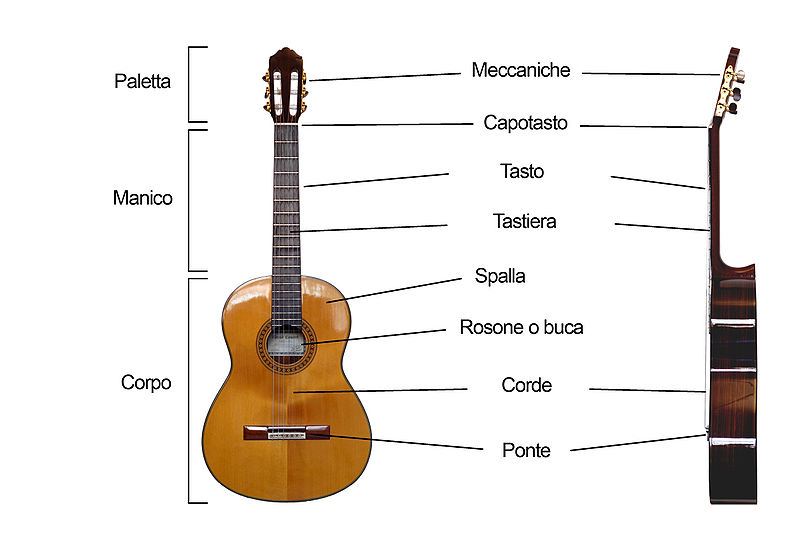
\includegraphics[scale=0.50]{./images/img14.jpg}
\end{figure}

\subsection{Corde}
Le corde delle chitarre moderne sono sei e sono ordinate dall'alto verso il basso nel seguente modo:
\begin{itemize}
	\item la prima corda corrisponde alla nota \textit{Mi cantino} (e);
	\item la seconda corrisponde alla nota \textit{Si} (B);
	\item la terza corrisponde alla nota \textit{Sol} (G);
	\item la quarta corrisponde alla nota \textit{Re} (D);
	\item la quinta corrisponde alla nota \textit{La} (A);
	\item la sesta corrisponde alla nota \textit{Mi basso} (E).
\end{itemize}
L'ultima corda dell'elenco è quella più spessa, mentre la prima è la più sottile.
\subsection{Tasti}
Sul manico della chitarra c’è la tastiera. Si chiama tastiera proprio perchè ci sono i tasti. Quest'ultimi sono delimitati da delle barrette di metallo e ognuno di essi corrisponde a una nota. Dunque, se abbiamo una chitarra a diciannove tasti, possiamo fare diciannove note diverse per ogni corda.\\
La distanza tra due tasti della stessa corda prende il nome di \textbf{semitono}. Ad esempio, se premiamo la sesta corda in corrispondenza del \textit{La}, poi premendo la corda al tasto adiacente più vicino alla cassa di risonanza (un semitono più alto) ascolteremo un \textit{La\#}.\\
Se non premiamo nessun tasto la corda si dice che è suonata a vuoto. Le sei corde suonate a vuoto devono emettere dei suoni ben precisi. Dunque, la chitarra deve essere accordata. L'accordatura classica delle sei corde, ovvero la nota che devono suonare le corde a vuoto (dal basso all'alto), è la seguente: \textit{Mi}, \textit{La}, \textit{Re}, \textit{Sol}, \textit{Si}, \textit{Mi}.\\
Conoscendo il suono prodotto dalle sei corde suonate a vuoto e sapendo che ogni nota suonata ad un tasto dista di un semitono dalla nota suonata al tasto adiacente possiamo mappare tutta la tastiera della chitarra.
\begin{figure}[H]
	\centering
	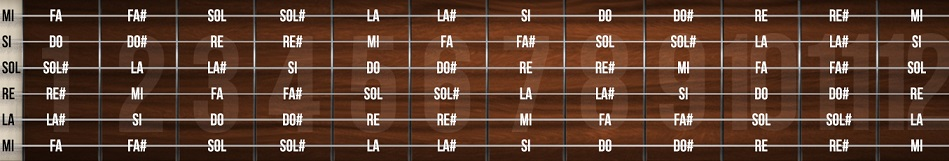
\includegraphics[scale=0.60]{./images/img13.jpg}
\end{figure}

\subsection{Tab}
La \textit{tab} è una rappresentazione delle corde della chitarra. Una tablatura è solitamente scritta usando sei linee orizzontali, ognuna corrispondente a una corda.\\
Al contrario dei normali spartiti, su una tablatura non ci sono le note da suonare ma si trovano le indicazioni su dove mettere le dita. I numeri sulle linee corrispondono ai tasti della tastiera. Ad esempio, un "1" sulla prima corda, indica di suonare il \textit{Mi cantino} tenendo premuto il primo tasto.
Se il numero è maggiore o uguale a uno, bisogna premere il tasto corrispondente quando si suonerà quella corda. Se troviamo uno \textbf{zero} allora si suona la corda a vuoto, senza premere alcun tasto.
\begin{figure}[H]
	\centering
	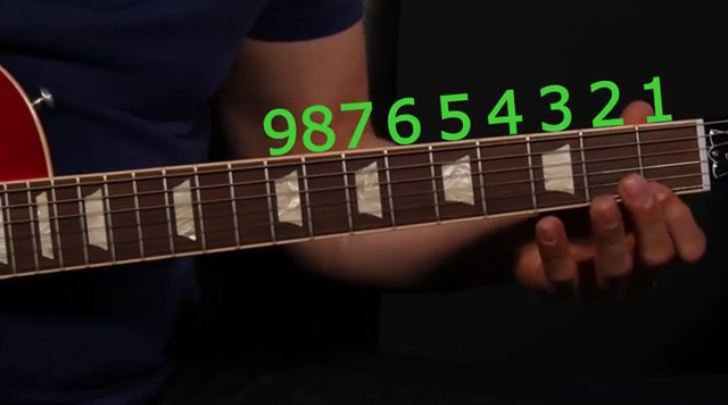
\includegraphics[scale=0.50]{./images/img15.png}
\end{figure}

Spesso leggendo una tablatura si trovano dei numeri che sono allineati verticalmente. In questo caso si premono più tasti contemporaneamente. Le \textit{tab} vanno lette come libri cioè da sinistra a destra.
\begin{figure}[H]
	\centering
	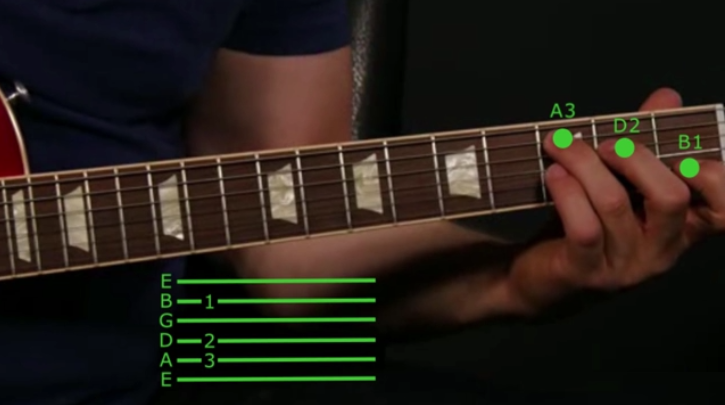
\includegraphics[scale=0.50]{./images/img16.png}
\end{figure}
    
    \chapter{Trasformata a Q Costante}
    \label{CH:Teoria}
    Le note musicali si possono classificare nel seguente modo:
\begin{figure}[H]
	\centering
	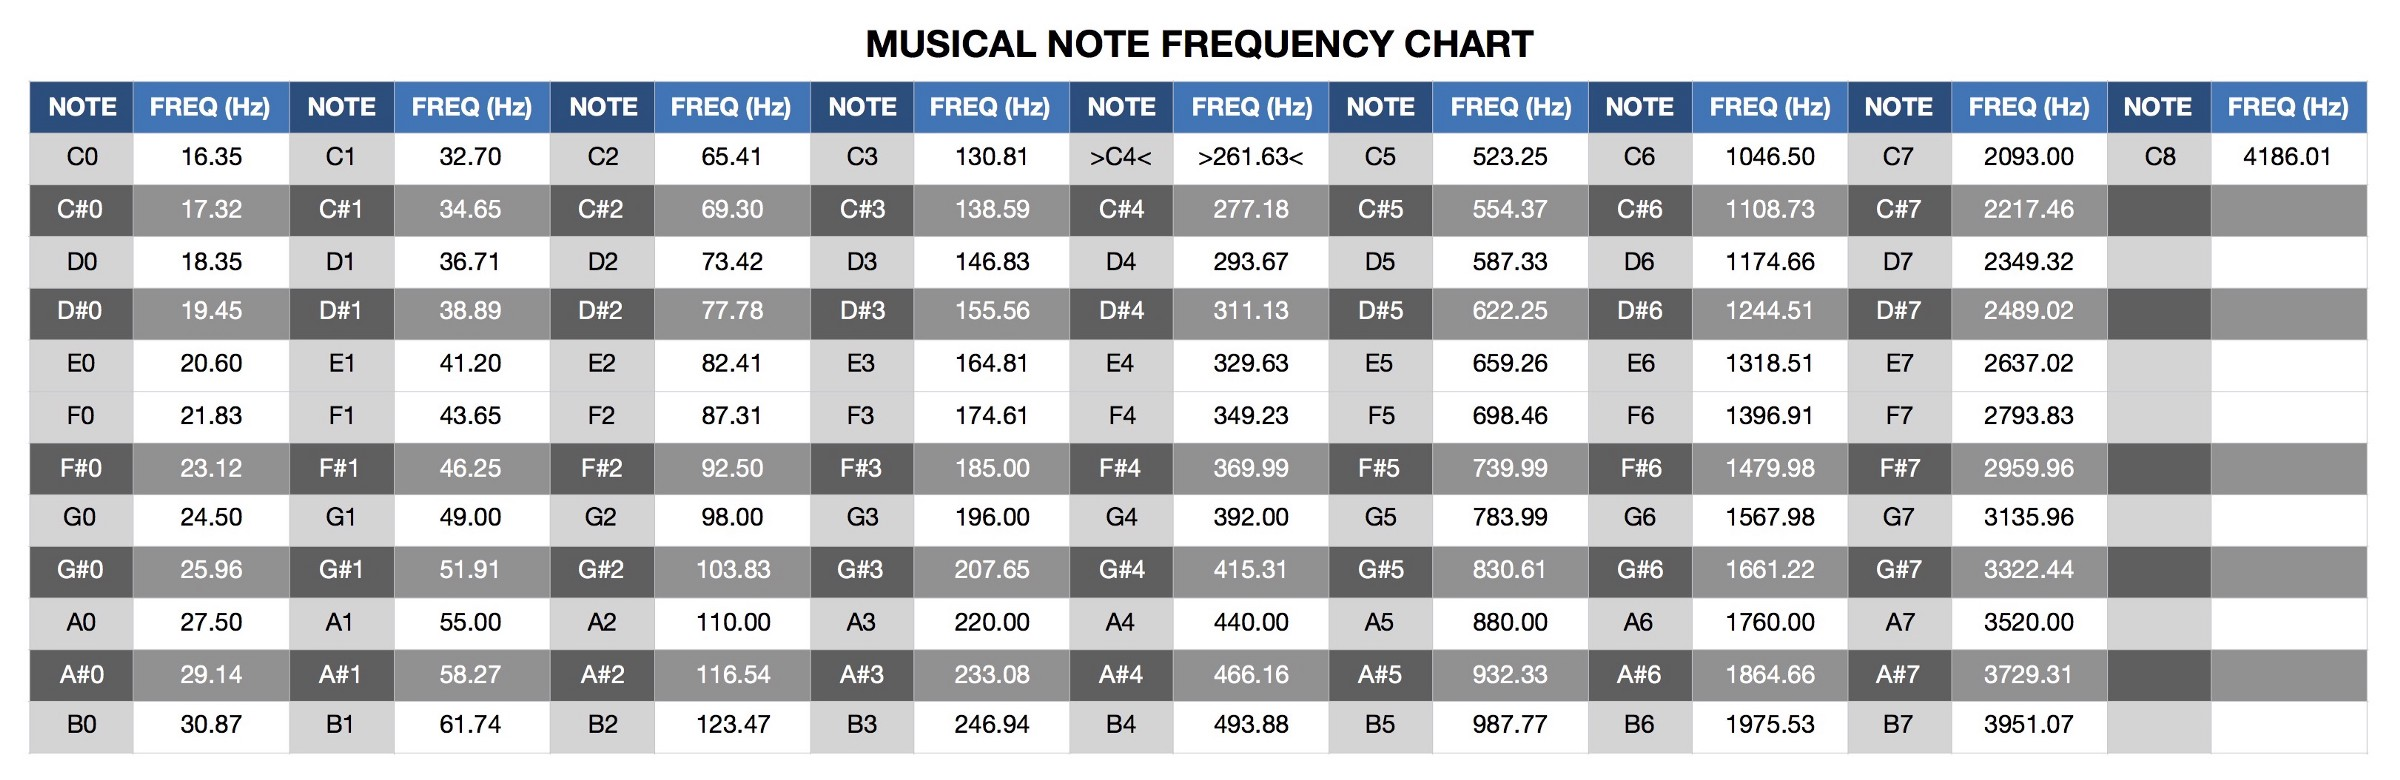
\includegraphics[scale=0.15]{./images/img4.jpg}
\end{figure}
La lettera a sinistra identifica la nota musicale mentre il numero a destra rappresenta la sua frequenza.

In musica, un'\textbf{ottava} è l'intervallo di otto note posizionate a frequenza diversa nella scala musicale. Le frequenze intermedie sono altre sei note. Per esempio, il \textit{La3} (A4) ha frequenza di 440 Hz, il \textit{la} posto un'ottava sopra ha frequenza 880 Hz, quello un'ottava sotto ha frequenza 220 Hz.

Se si rappresentassero le prime sei ottave della nota C potremmo vedere che la sua frequenza raddoppia ad ogni ottava. \\
\newline
I tasti che intercorrono fra gli estremi della stessa ottava (esempio \textit{Do3}-\textit{Do4}) sono dodici note per cui la frequenza deve raddoppiare ogni dodici note. Si può rappresentare quanto detto dalla seguente formula: \\

\begin{center}
	\begin{math}
		F_{k}=440Hz \cdot 2^{k \over 12}
	\end{math}
\end{center}
Nel campo della musica viene utilizzata la trasformata a Q costante, a discapito della più nota trasformata di Fourier, proprio per la sua natura esponenziale. Inoltre, l'accuratezza della trasformata a Q costante è analoga alla scala logaritmica e imita l'orecchio umano, avendo una risoluzione di frequenza più alta a quelle più basse e una risoluzione più bassa alle frequenze più alte. Infatti, dal seguente grafico si può notare la natura esponenziale della funzione:
\begin{center}
	\begin{tikzpicture}
	\begin{axis}[ 
		xlabel=$k$,
		ylabel={$frequenza$}
		] 
		\addplot {440*2^x/12}; 
	\end{axis}
\end{tikzpicture}
\end{center}
    
    \chapter{Architettura e addestramento del modello}
    \label{CH:Val_num}
    I problemi che verranno segnalati nel seguente capitolo non si sono presentati subito, ma solo quando si è testata l'accuratezza del modello per cui ci sono paragrafi in cui si parla di esso senza averlo ancora definito.
\section{Machine learning}
Usare un algoritmo scritto da un programmatore non è sempre la soluzione migliore in quanto bisogna definire tutti i parametri e i dati necessari alla risoluzione del problema. Infatti, esiste anche un'altra strategia cioè quella di far imparare ad una macchina come risolverlo. La prima cosa che viene spontaneo chiedersi è: come fa una macchina ad imparare? Gli psicologi ci insegnano che l’apprendimento consiste nell’acquisizione o modifica di conoscenze, comportamenti, abilità, valori ed esperienze che sono poi utilizzati per vivere la vita di tutti i giorni. Tramite l’apprendimento creiamo delle regole generali che sono assimilabili in modelli di apprendimento. Questi modelli ci indicano come comportarci in una determinata situazione, ad interagire con gli altri, come leggere, come socializzare e così via. L’apprendimento è un processo iterativo, che continua per tutta la vita e ci permette di migliorare le nostre conoscenze a seconda delle informazioni che raccogliamo. Lo stesso fanno le macchine: dai dati di \textit{input} che analizzano ricavano i modelli di apprendimento.\\
\newline
\section{Librerie utilizzate}
I \textit{package} usati per realizzare il progetto sono:
\begin{itemize}
	\item \textit{numpy, versione 1.17.4}, è una libreria che aggiunge supporto a grandi matrici e \textit{array} multidimensionali insieme a una vasta collezione di funzioni matematiche di alto livello per poter operare efficientemente su queste strutture dati;
	\item \textit{jams, versione 0.3.4}, è una libreria che legge file \textit{JSON} inerenti al mondo della musica;
	\item \textit{librosa, versione 0.8.0}, è una libreria per la musica e l'analisi audio. Fornisce gli elementi necessari per recuperare informazioni musicali;
	\item \textit{scipy, versione 1.4.1}, è una libreria di algoritmi e strumenti matematici che contiene moduli per l'ottimizzazione, per l'algebra lineare, elaborazione di segnali ed immagini e altro;
	\item \textit{matplotlib, versione 3.1.2}, è una libreria per la creazione di grafici;
	\item \textit{tensorflow, versione 2.1.0}, è una libreria utilizzata per il \textit{machine learning} che fornisce moduli sperimentati e ottimizzati, utili nella realizzazione di algoritmi per diversi tipi di compiti percettivi e di comprensione del linguaggio;
	\item \textit{keras, versione 2.3.1}, consente di implementazione algoritmi basati su reti neurali. Permette di sviluppare e prototipare in maniera semplice e veloce modelli nell’ambito del \textit{machine learning} e del \textit{deep learning}. Supporta come \textit{back-end} \textit{Tensorflow} ed è integrata in esso dalla versione 2.
\end{itemize}

\section{Set dati GuitarSet}
Fortunatamente, su Internet abbiamo trovato un \textit{dataset} di file audio di chitarra già pronto su cui lavorare. Il \textit{GuitarSet}, chiamato così dal suo creatore, è costituito dai file audio e dai suoi \textit{tab}.\\
\newline
Questo \textit{dataset} contiene trecentosessanta estratti di canzoni della durata di circa trenta secondi l'uno. Quest'ultime sono suonate da sei persone diverse che leggono gli stessi fogli musicali. I fogli musicali sono generati da una combinazione di:
\begin{itemize}
	\item \textbf{5 stili}: rock, cantautore, bossa nova, jazz e funk;
	\item \textbf{3 progressioni}: dodici bar blues, autumn leaves e pachelbel canon;
	\item \textbf{2 Tempi}: lento e veloce.
\end{itemize}
Gli estratti sono registrati sia con il \textit{pickup esafonico} che con un microfono a condensatore \textit{Neumann U-87}.
Ci sono tre registrazioni audio per ogni estratto:
\begin{itemize}
	\item \textbf{hex}: file .\textit{wav} originali a sei canali dal \textit{pickup esafonico};
	\item \textbf{hex\_cln}: file .\textit{wav} con rimozione delle interferenze applicata;
	\item \textbf{mic}: registrazione monofonica dal microfono di riferimento.
\end{itemize}
Noi abbiamo usato registrazioni di tipo \textbf{mic} perchè sono quelle che più si avvicinano al caso delle registrazioni tramite microfono dello \textit{smartphone}.\\
\newline
Ciascuno dei trecentosessanta estratti ha anche un file .\textit{jams} che memorizza sedici annotazioni:
\begin{itemize}
	\item Intonazione:
	\begin{itemize}
		\item 6 annotazioni \textit{pitch\_contour} (1 per stringa)
		\item 6 annotazioni \textit{midi\_note} (1 per stringa)
	\end{itemize}
	\item Beat e tempo:
	\begin{itemize}
		\item 1 annotazione \textit{beat\_position}
		\item 1 annotazione del tempo
	\end{itemize}
	\item Accordi:
	\begin{itemize}
		\item 2 annotazioni di accordi (istruite ed eseguite)
	\end{itemize}
\end{itemize}
Noi useremo le annotazioni \textit{midi\_note}, da cui prenderemo le \textit{tab}.
\subsection{Ricavare le tab dai file .jams}
Innanzitutto calcoliamo il numero di \textit{frame} per ogni \textit{file} audio, così da poter ricavare un'immagine completa e le corrispondenti \textit{tab} per ogni \textit{frame}. Per calcolare l'istante di tempo per ogni \textit{frame} utilizziamo la funzione \textit{get\_times()}:
\vspace*{2ex}
\pythonexternal{./codes/times.py}
\vspace*{2ex}
\noindent Adesso che, per ogni \textit{file} audio, abbiamo una divisione in \textit{frame} di cui conosciamo gli istanti di tempo esatti, possiamo estarre dai file .\textit{jams} del \textit{dataset} le \textit{tab} corrispondenti.\\ Più precisamente, dai file .\textit{jams} prendiamo le note \textit{MIDI} e creiamo una matrice 6x19 dove il sei rappresenta il numero di corde mentre il diciannove rappresenta il numero di tasti.
\vspace*{2ex}
\begin{figure}[H]
	\centering
	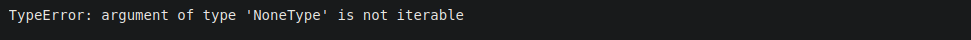
\includegraphics[scale=0.65]{./images/img11.png}
\end{figure}
\noindent Ogni tasto della matrice ha un valore \textit{MIDI} che varia da 40 a 82.
\vspace*{2ex}
\pythonexternal{./codes/matrixMidi.py}
\vspace*{2ex}
\noindent Ad ogni matrice sostituiamo i valori \textit{MIDI} con una matrice della stessa dimensione in cui ci sono solo uni o zeri a seconda dei valori \textit{MIDI} che il \textit{file} .\textit{jams} ci ha restituito. Ad esempio, dato un \textit{frame}, se dal file .\textit{jams} leggiamo che sono state suonate le note 40 della sesta corda, 60 della seconda corda e 67 della prima, avremo la seguente matrice:
\vspace*{2ex}
\pythonexternal{./codes/matrixUniZeri.py}
\noindent Queste matrici, da ora in avanti, saranno chiamate \textit{labels} e verranno usate come \textit{target y} del modello, per questo è molto importante avere una mappatura di numeri interi "categorica", per cui useremo la codifica \textit{one-hot}, cioè si può trovare un solo "1" in ogni riga. Per finire, aggiungiamo altre due colonne in testa alle labels che serviranno a capire se la corda è stata suonata o meno (colonna 0) e se si, se è stata suonata a vuoto oppure o no (colonna 1).\\
\newline
Di conseguenza, la matrice finale di dimensione 6x21 è la seguente:
\vspace*{2ex}
\pythonexternal{./codes/matrixUniZeriFinale.py}
\vspace*{2ex}
\noindent Il codice che esegue quanto abbiamo appena descritto è il seguente:
\vspace*{2ex}
\pythonexternal{./codes/labels.py}
\subsection{Ricavare le immagini dai file audio}
Dopo esserci ricavati le \textit{labels} per ogni \textit{frame}, dobbiamo trovare un modo per far "imparare" al modello che un frammento di audio sia associato al corrispondente \textit{label}.
Grazie alla libreria \textit{librosa} possiamo analizzare e manipolare il suono, vedere lo spettrogramma della trasformata a Q costante e ricavare per ogni \textit{file} audio un'immagine.\\
Per esempio, questo è lo spettrogramma della trasformata a Q costante di un audio del \textit{dataset}.
\begin{figure}[H]
	\centering
	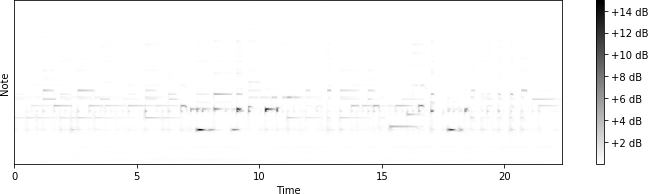
\includegraphics[scale=0.60]{./images/img7.png}
\end{figure}
\noindent Per utilizzare al meglio il modulo \textit{librosa.cqt()}, dobbiamo impostare alcuni parametri:
\begin{itemize}
	\item \textbf{sr\_downs}: il numero di campioni al secondo del segnale di ingresso;
	\item \textbf{hop\_length}: il numero di campioni tra i fotogrammi;
	\item \textbf{n\_bins}: il numero di bande di frequenza nello spettrogramma risultante;
	\item \textbf{bins\_per\_octave}: il numero di bande di frequenza per ogni ottava.
\end{itemize}
\textbf{Problemi riscontrati:} le funzioni per caricare il \textit{file} audio e la \textit{cqt} restitiscono dei valori negativi e non scalati, per questo bisogna effettuare delle operazioni sulle matrici che potrebbero alterare il risultato. Inoltre, la scelta dei parametri di \textit{simple rate} e \textit{n\_bins} influenzano l'accuratezza del modello. \\
\newline
\textbf{Soluzioni provate:}
\begin{itemize}
	\item Abbiamo avuto la necessità di scrivere delle funzioni per convertire i valori della matrice calcolata. Dunque, è stata ridimensionata in modo che si trovi nell'intervallo 0-255 e poi normalizzata nell'intervallo 0-1;
	\item All'inizio l'audio è stato campionato a 44100Hz perchè è la stessa frequenza usata nel \textit{dataset}. Le immagini generate avevano una frequenza delle note maggiore di quella che avrebbero dovuto avere. Infatti, nella figura in alto la parte scura era meno spessa. Questo provocava delle imprecisioni perchè la rete non riusciva a riconoscere la nota corretta;
	\item Il valore iniziale scelto di \textit{n\_bins} è stato 96. Questo influenzava le dimensioni dell'immagine in quanto è il valore della sua lunghezza e risultava troppo piccola.
\end{itemize}
\textbf{Soluzione finale:} le scelte finali sono ricadute rispettivamente su 22050Hz come \textit{simple rate} e su 192 come \textit{n\_bins} perchè dopo aver effettuato diverse ricerche, in ambito di manipolazione del suono, è consigliato utilizzare questi valori. Per quanto riguarda il ridimensionamento abbiamo usato le funzioni \textit{librosa.util.normalize()} e \textit{np.abs()} subito dopo aver caricato i file audio invece di manipolare le matrici in seguito.
\vspace*{2ex}
\pythonexternal{./codes/librosa.py}
\vspace*{2ex}
\noindent In particolare, una volta che l'audio è un oggetto dati \textit{librosa}, \textit{Python} lo vede come un numpy \textit{array} e quindi possiamo evitare di salvarci fisicamente dei classici \textit{file} immagini \textit{.jpeg} o \textit{.png} e continuare a lavorare con le matrici.\\
\newline
I dati (\textit{images} e \textit{labels}) di ogni \textit{file} audio sono stati compressi in archivi .\textit{npz} per organizzare meglio il \textit{dataset} da dare come \textit{input} al modello.
\vspace*{2ex}
\pythonexternal{./codes/store.py}
\vspace*{2ex}
\subsection{Pre-elaborare i dati}
Carichiamo i \textit{file} .\textit{npz} salvati in precedenza.\\
\newline
\textbf{Problemi riscontrati:} mentre lavoravamo con il modello ci siamo resi conto che usare una finestra di 1s risultava essere troppo ampia. Se nell'immagine ci sono troppe note e la rete deve riconoscerne poche, non riesce a farlo. Infatti, se non viene scelta  correttamente la finestra, l'accuratezza del modello è molto bassa e dopo appena 15 epoche la rete non tende più ad imparare.
\begin{figure}[H]
	\centering
	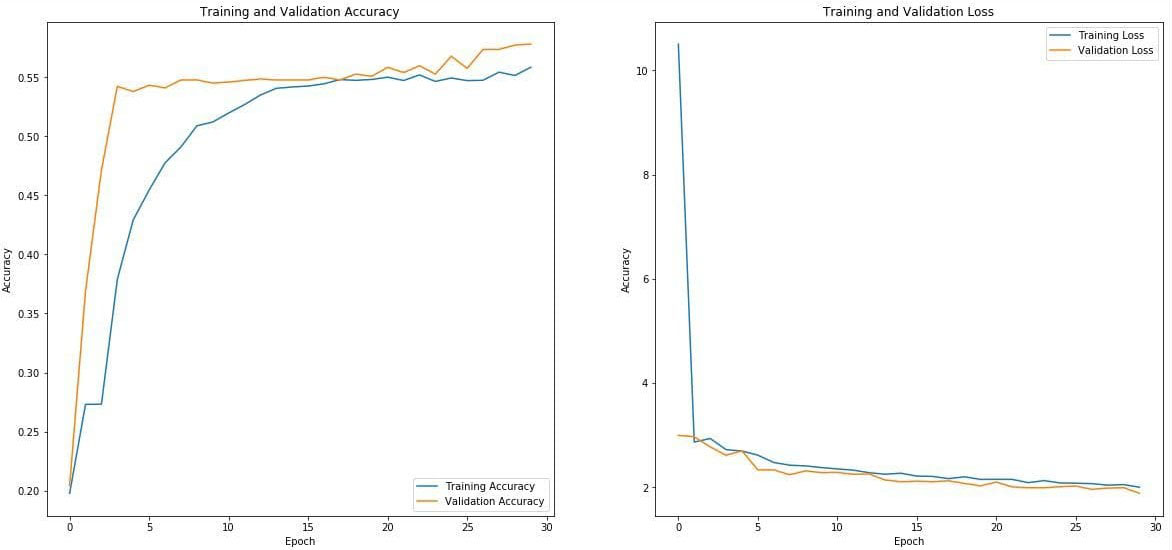
\includegraphics[scale=0.5]{./images/img28.jpg}
\end{figure}
\textbf{Soluzioni provate:}
\begin{itemize}
	\item Abbiamo provato finestre di grandezza compresa tra 0.1s e 0.3s.
\end{itemize}
\textbf{Soluzione finale:} si è visto, sperimentalmente, che un buon arco di tempo per riconoscere una nota è 200ms che, nel nostro caso, corrispondono ad una finestra di nove righe della matrice dell'immagine.\\
\newline
Di conseguenza, quello che dobbiamo fare non è altro che associare, per ogni \textit{frame}, una \textit{label} e un'\textit{immagine} di nove righe (192x9), senza dimenticare di aggiungere un \textit{padding} (quattro zeri nell'\textit{array}, sia all'inizio che alla fine, con la funzione \textit{np.pad()}) perchè così l'ultimo valore, della finestra di nove righe, risulta essere congruo con gli altri.\\
\newline
\begin{figure}[H]
	\centering
	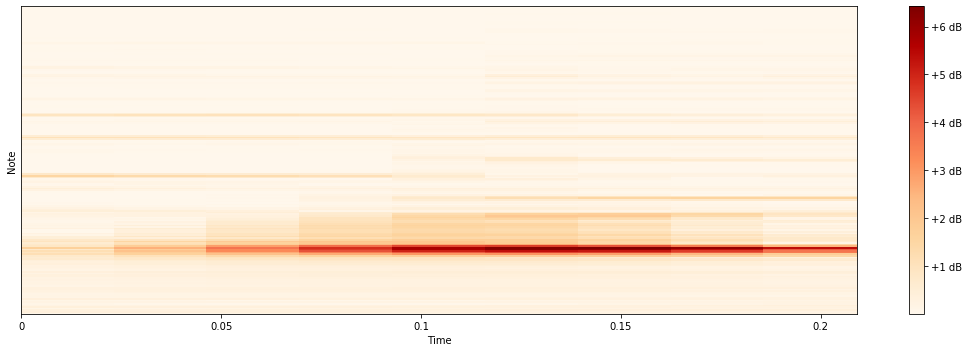
\includegraphics[scale=0.40]{./images/img8.png}
\end{figure}
\noindent Il codice che esegue quanto abbiamo appena descritto è il seguente:
\vspace*{2ex}
\pythonexternal{./codes/preElaborazionedati1.py}
\vspace*{2ex}
Una volta ottenuto l'\textit{array}, chiamato (\textit{training\_data}), di tutte le \textit{images} e i \textit{labels} dei \textit{file} audio, e assegnati rispettivamente le variabili \textit{X} e \textit{y}, lo mescoliamo in modo da avere più imprevedibilità. Infine, suddividiamo questi dati nel seguente modo:
\begin{itemize}
	\item 10\% dei dati li usiamo per la \textit{validation}
	\item 10\% dei dati li usiamo per i \textit{test}
	\item 80\% dei dati li usiamo per il \textit{traning}
\end{itemize}
Il \textit{traning set} lo utilizziamo per costruire il modello, il \textit{validation set} per validare i parametri dei \textit{layer} della rete neurale mentre il \textit{test set} per determinare l'accuratezza.\\
\newline
Il codice è il seguente:
\vspace*{2ex}
\pythonexternal{./codes/preElaborazionedati2.py}
\vspace*{2ex}
\section{Modello della rete}
La difficoltà nell’apprendere i meccanismi di implementazione su \textit{Keras} sono ridotti al minimo grazie alla vasta documentazione presente, arricchita da numerosi esempi sulle più utilizzate configurazioni inerenti il \textit{machine learning}, come le \textit{CNN} (Convolutional Neural Network).
Le operazioni di calcolo matriciali possono essere accelerate sia tramite \textit{CPU}, che \textit{GPU} (su \textit{hardware} \textit{Nvidia} con supporto \textit{CUDA}). Nel nostro caso è stata utilizzata una \textit{GPU} in modo da sfruttare direttamente la sua potenza parallela contenute nelle schede video recenti.
\vspace*{2ex}
\pythonexternal{./codes/gpu.py}
\vspace*{2ex}
\noindent Le caratteristiche e i vantaggi che ci hanno portato ad utilizzare \textit{Keras} nell’ambito del progetto sono:
\begin{itemize}
	\item \textbf{semplicità}: a differenza di altre \textit{API}, è possibile realizzare modelli complessi scrivendo meno righe di codice, mantenendo nel contempo chiarezza nello sviluppo. Tutto ciò consente allo sviluppatore di mantenere nel tempo il codice in maniera agevole;
	\item \textbf{modularità}: un modello in \textit{Keras} è inteso come una sequenza o un grafo di singoli, compatti e completamente configurabili moduli, che possono lavorare in sinergia tra loro con il minimo numero di restrizioni possibili. Ciò rende il codice estremamente flessibile;
	\item \textbf{estensibilità}: in base alle esigenze dello sviluppatore, è possibile aggiungere facilmente nuovi moduli (ad esempio classi e funzioni) ad un progetto preesistente.
\end{itemize}
\subsection{Uso di Keras}
Prima di dare in \textit{input} al modello il \textit{traning set} e il \textit{validation set}, dobbiamo fare delle modifiche alla dimensione del numpy \textit{array} delle immagini \textit{X} in quanto il modello si aspetta una dimensione di \textit{input} di \textit{BATCH} x 192 x 9 x 1.
\begin{itemize}
	\item \textit{BATCH} sono la quantità di valori dell'intero \textit{training set};
	\item 192 è l'altezza dell'immagine (H);
	\item 9 è la lunghezza dell'immagine (W);
	\item 1 ci indica che l'immagine è in bianco e nero.
\end{itemize}
La \textit{y} non ha bisogno di modifiche perchè le dimensioni sono già quelle corrette cioè ha dimensione \textit{BATCH} x 21 x 6.\\
\newline
Il codice che esegue quanto abbiamo appena descritto è il seguente:
\vspace*{2ex}
\pythonexternal{./codes/modelloFinale1.py}
\vspace*{2ex}
A questo punto definiamo il modello con l'aggiunta dei seguenti \textit{layers}:
\begin{itemize}
	\item \textbf{Conv2D}: mette in evidenza le caratteristiche interessanti dell'immagine. Parametri di \textit{input}: numero di filtri, grandezza filtri, \textit{input shape} e funzione di attivazione;
	\item \textbf{MaxPooling2D}: riduce la dimensione dell'immagine, elimina le informazioni inutili mantenendo quelle più importanti;
	\item \textbf{Dropout}: elimina una percentuale di dati casuali. Ad esempio, elimina rumori di sottofondo e mantiene le informazioni più importanti;
	\item \textbf{Flattern}: appiattisce il tensore e rimuove tutte le dimensioni;
	\item \textbf{Dense}: crea un \textit{layer} di neuroni, ognuno dei quali connesso ad ogni uscita del \textit{layer} precedente;
	\item \textbf{Reshape}: determina la dimensione di uscita. In questo caso è 6x21;
	\item \textbf{Activation}: la funzione di attivazione è una "porta" matematica tra l'\textit{input} che alimenta il neurone corrente e il suo \textit{output} che va allo strato successivo.
\end{itemize}
L'unità lineare rettificata (\textit{ReLU}) è la funzione di attivazione più comunemente utilizzata nel \textit{deep learning}. La funzione restituisce 0 se l'\textit{input} è negativo, ma per qualsiasi \textit{input} positivo, restituisce quel valore.\\
La funzione \textit{softmax} è molto utilizzata in statistica e consente di gestire un vettore di uscita normalizzato di n elementi, dove ogni elemento può valere da 0 ad 1 e la somma di tutti gli elementi è pari ad 1. In sostanza il nostro vettore di uscita sarà in una forma simile a quella \textit{one-hot} e ogni posizione corrisponderà alla probabilità (normalizzata) che l’immagine appartenga a quella specifica classe. La somma di tutte le probabilità sarà 1 = 100\%.
\begin{figure}[H]
	\centering
	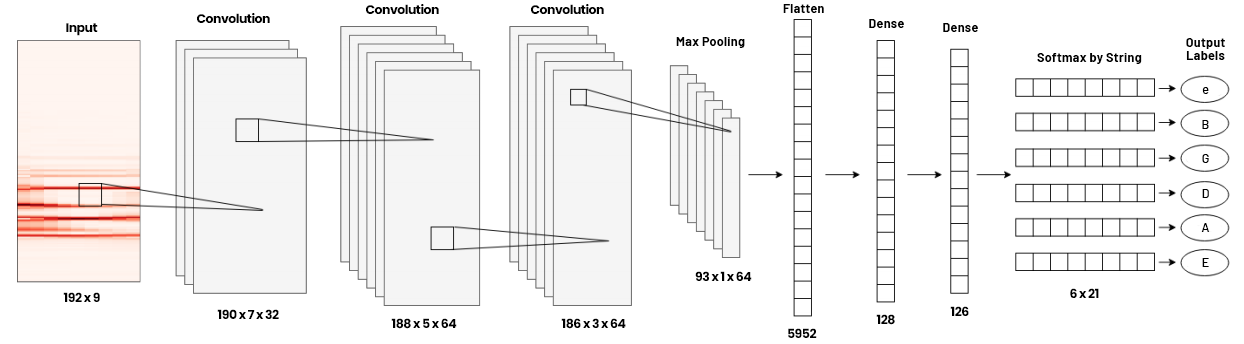
\includegraphics[scale=1.4]{./images/model.png}
\end{figure}
\noindent Per compilare il modello abbiamo scelto come ottimizzatore l'algoritmo \textit{Adadelta} che utilizza un metodo di discesa del gradiente stocastico basato sul tasso di apprendimento adattivo per dimensione per affrontare l'inconveniente del continuo declino dei tassi di apprendimento durante la formazione e la necessità di un tasso di apprendimento globale selezionato manualmente.\\
Il codice è il seguente:\\
\newline
\vspace*{2ex}
\pythonexternal{./codes/modelloFinale3.py}
\vspace*{2ex}
\noindent La funzione \textit{summary()} ci descrive il modello:
\vspace*{2ex}
\pythonexternal{./codes/modelloFinale5.py}
\vspace*{2ex}
\noindent In particolare, per il modello abbiamo usato delle funzioni personalizzate per la funzione di attivazione finale del modello (\textit{sofmax\_by\_string}), per la funzione obiettivo \textit{loss} (\textit{catcross\_by\_string}) e per le metriche di accuratezza (\textit{avg\_acc}) che devono essere valutate dal modello durante l'addestramento.\\
Esse permettono di utilizzare la funzione di attivazione \textit{softmax} e la funzione di perdita \textit{categorical\_crossentropy} per ogni stringa, e alla fine concatenare i sei risultati in un unico valore.\\
\newline
Il codice che esegue quanto abbiamo appena descritto è il seguente:
\vspace*{2ex}
\pythonexternal{./codes/modelloFinale2.py}
\vspace*{2ex}
\noindent Per avviare l'addestramento del modello eseguiamo la funzione \textit{model.fit()} dove indichiamo con \textit{batch\_size} il numero di campioni per ogni aggiornamento del gradiente e con \textit{epochs} il numero di iterazioni sul quale il modello deve effettuare il \textit{training}. In questo modo partirà la fase di addestramento che andrà ad affinare sempre di più le performance del modello.\\
\newline
Il codice che esegue quanto abbiamo appena descritto è il seguente:
\vspace*{2ex}
\pythonexternal{./codes/modelloFinale4.py}
\subsection{Addestramento del modello}
Dopo diverse prove sperimentali, abbiamo deciso di eseguire il modello per cinquecento epoche:
\begin{figure}[H]
	\centering
	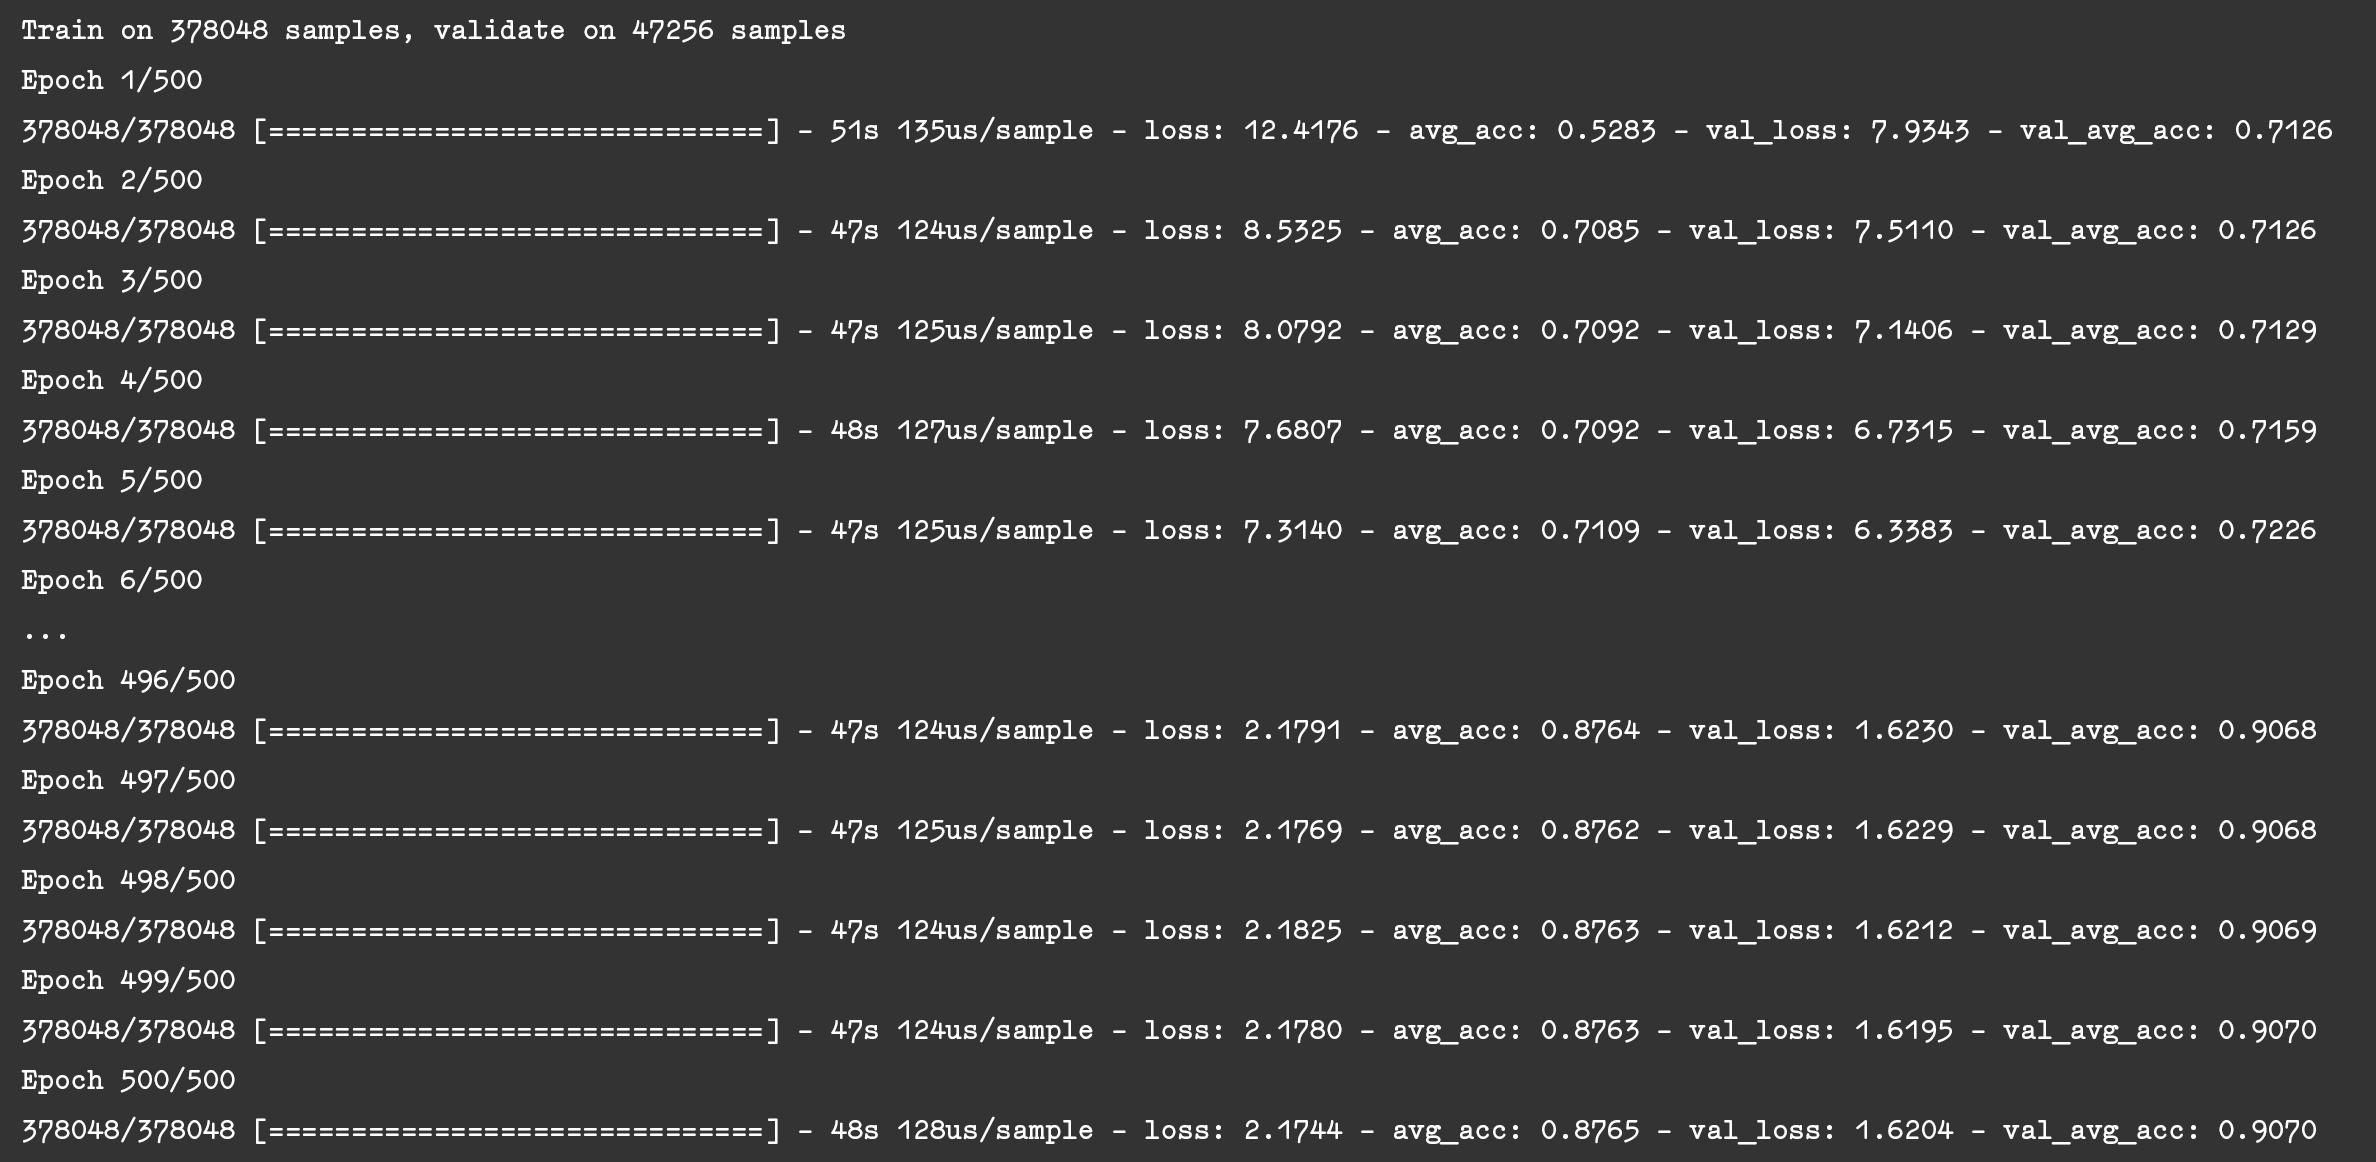
\includegraphics[scale=0.8]{./images/storia.png}
\end{figure}
\noindent Come si può notare dal \textit{log}, un’epoca (cioè l’addestramento eseguito su un intero \textit{dataset} di 378048 immagini) viene eseguita in circa 47 secondi, usando mediamente 124 microsecondi per immagine. Questo è il risultato ottenuto utilizzando una \textit{GPU NVIDIA RTX 2060}.\\
\newline
Questo modello raggiunge una precisione di circa 0,87 su 1 (o 87\%) e una perdita del 2\% sui dati di addestramento. Invece, sui dati di validazione la precisione supera lo 0,90 (90\%) e raggiunge una perdita del 1,6\% sui dati di validazione. I \textit{loss} sono la media delle perdite sui dati di \textit{batch} di addestramento.\\
\newline
Il grafico sottostante ci fa comprendere meglio i risultati:
\begin{figure}[H]
	\centering
	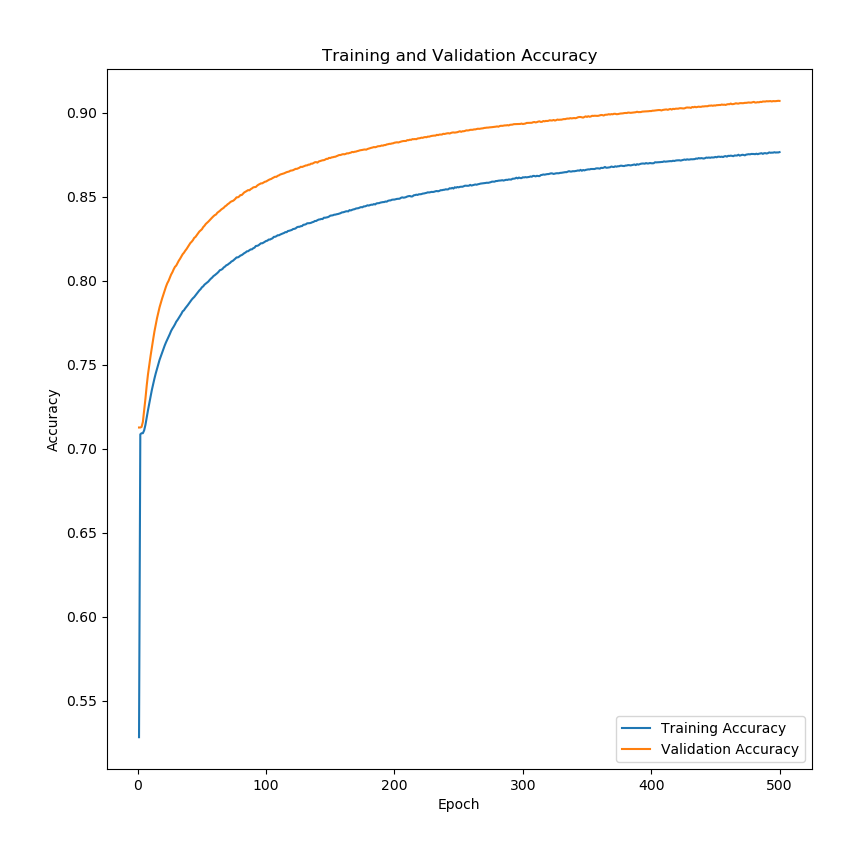
\includegraphics[scale=0.40]{./images/plot.png}
\end{figure}
\begin{figure}[H]
	\centering
	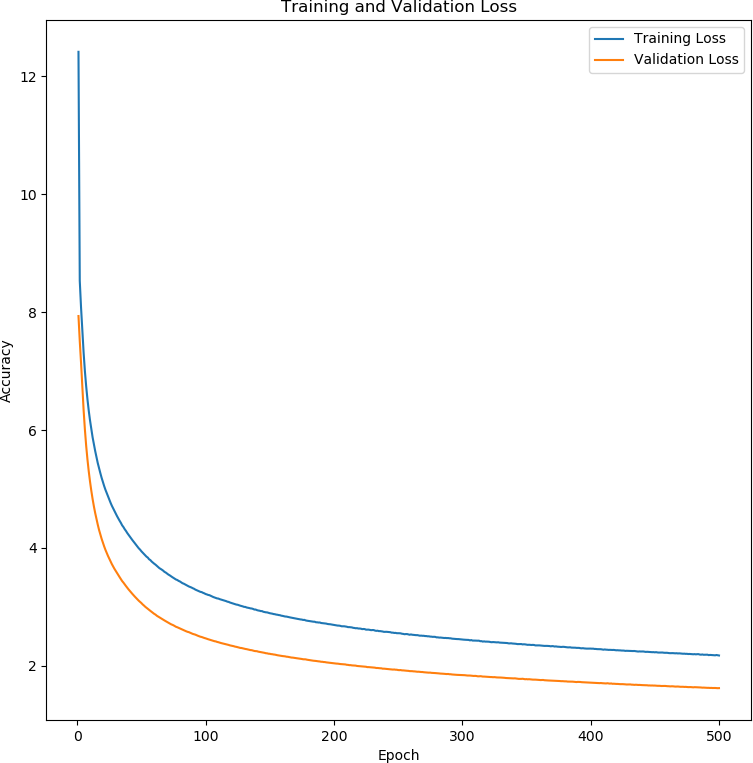
\includegraphics[scale=0.40]{./images/plot2.png}
\end{figure}

\section{Valutazione del modello}
Abbiamo eseguito diversi \textit{test} per mettere alla prova il modello utilizzando il \textit{training test}. La matrice \textit{Answer} è la \textit{y} corrispondente alla \textit{X} data come \textit{input} alla \textit{predict}. Invece, la \textit{Prediction} corrisponde all'\textit{output} della rete. Il valore più grande della riga corrisponde a dove secondo il modello ci debba essere "1".\\
\newline
Di seguito riportiamo un esempio:
\vspace*{2ex}
\pythonexternal{./codes/test.py}
\vspace*{2ex}
\noindent Abbiamo confrontato le prestazioni del modello sul \textit{dataset} di prova e i risultati sono stati quelli previsti. Infatti, l'accuratezza e la perdita dei dati di \textit{test} sono molto simili a quelli dei dati di validazione. Quello che otteniamo è un errore del 10\% (quindi un'\textit{accuracy} del 90\%).
\vspace*{2ex}
\pythonexternal{./codes/valutazione.py}
\vspace*{2ex}

Il codice che esegue quanto abbiamo appena descritto è il seguente:
\vspace*{2ex}
\pythonexternal{./codes/accuratezza.py}
\vspace*{2ex}
    
    \chapter{Implementazione su dispositivo Embedded}
    \label{CH:Val_num}
    Per dispositivo \textit{embedded} si intende un dispositivo piccolo e compatto con consumi energetici molto contenuti. Proprio per queste caratteristiche sono usati per il \textit{deployment} di reti neurali.\\
La scelta è caduta sui dispositivi mobili. Questa decisione è stata vincolante perchè disponevamo di solo queste risorse \textit{hardware}.

\section{Conversione del modello da Keras a Tensorflow Lite}
Abbiamo convertito il modello usando \textit{Tensorflow Lite}. Il seguente codice consente di caricare il modello addestrato tramite \textit{Tensorflow} e di convertirlo nel formato .\textit{tflite} pronto per essere utilizzato su un dispositivo \textit{embedded}.
\vspace*{2ex}
\pythonexternal{./codes/tensorflowLite.py}
\noindent Il convertitore ha il compito di ottimizzare il modello riducendo le sue dimensioni e aumentando la sua velocità di esecuzione.
\section{Sviluppo applicazione Android}
\subsection{Sviluppo applicazione con Java 1.8 e Android Studio 4.1.2}
\textit{Java} è una piattaforma che consente di eseguire i programmi scritti in questo linguaggio.\\
\newline
\textit{Android Studio} è un ambiente di sviluppo integrato per lo sviluppo per la piattaforma \textit{Android}.\\
\newline
\begin{figure}[H]
	\centering
	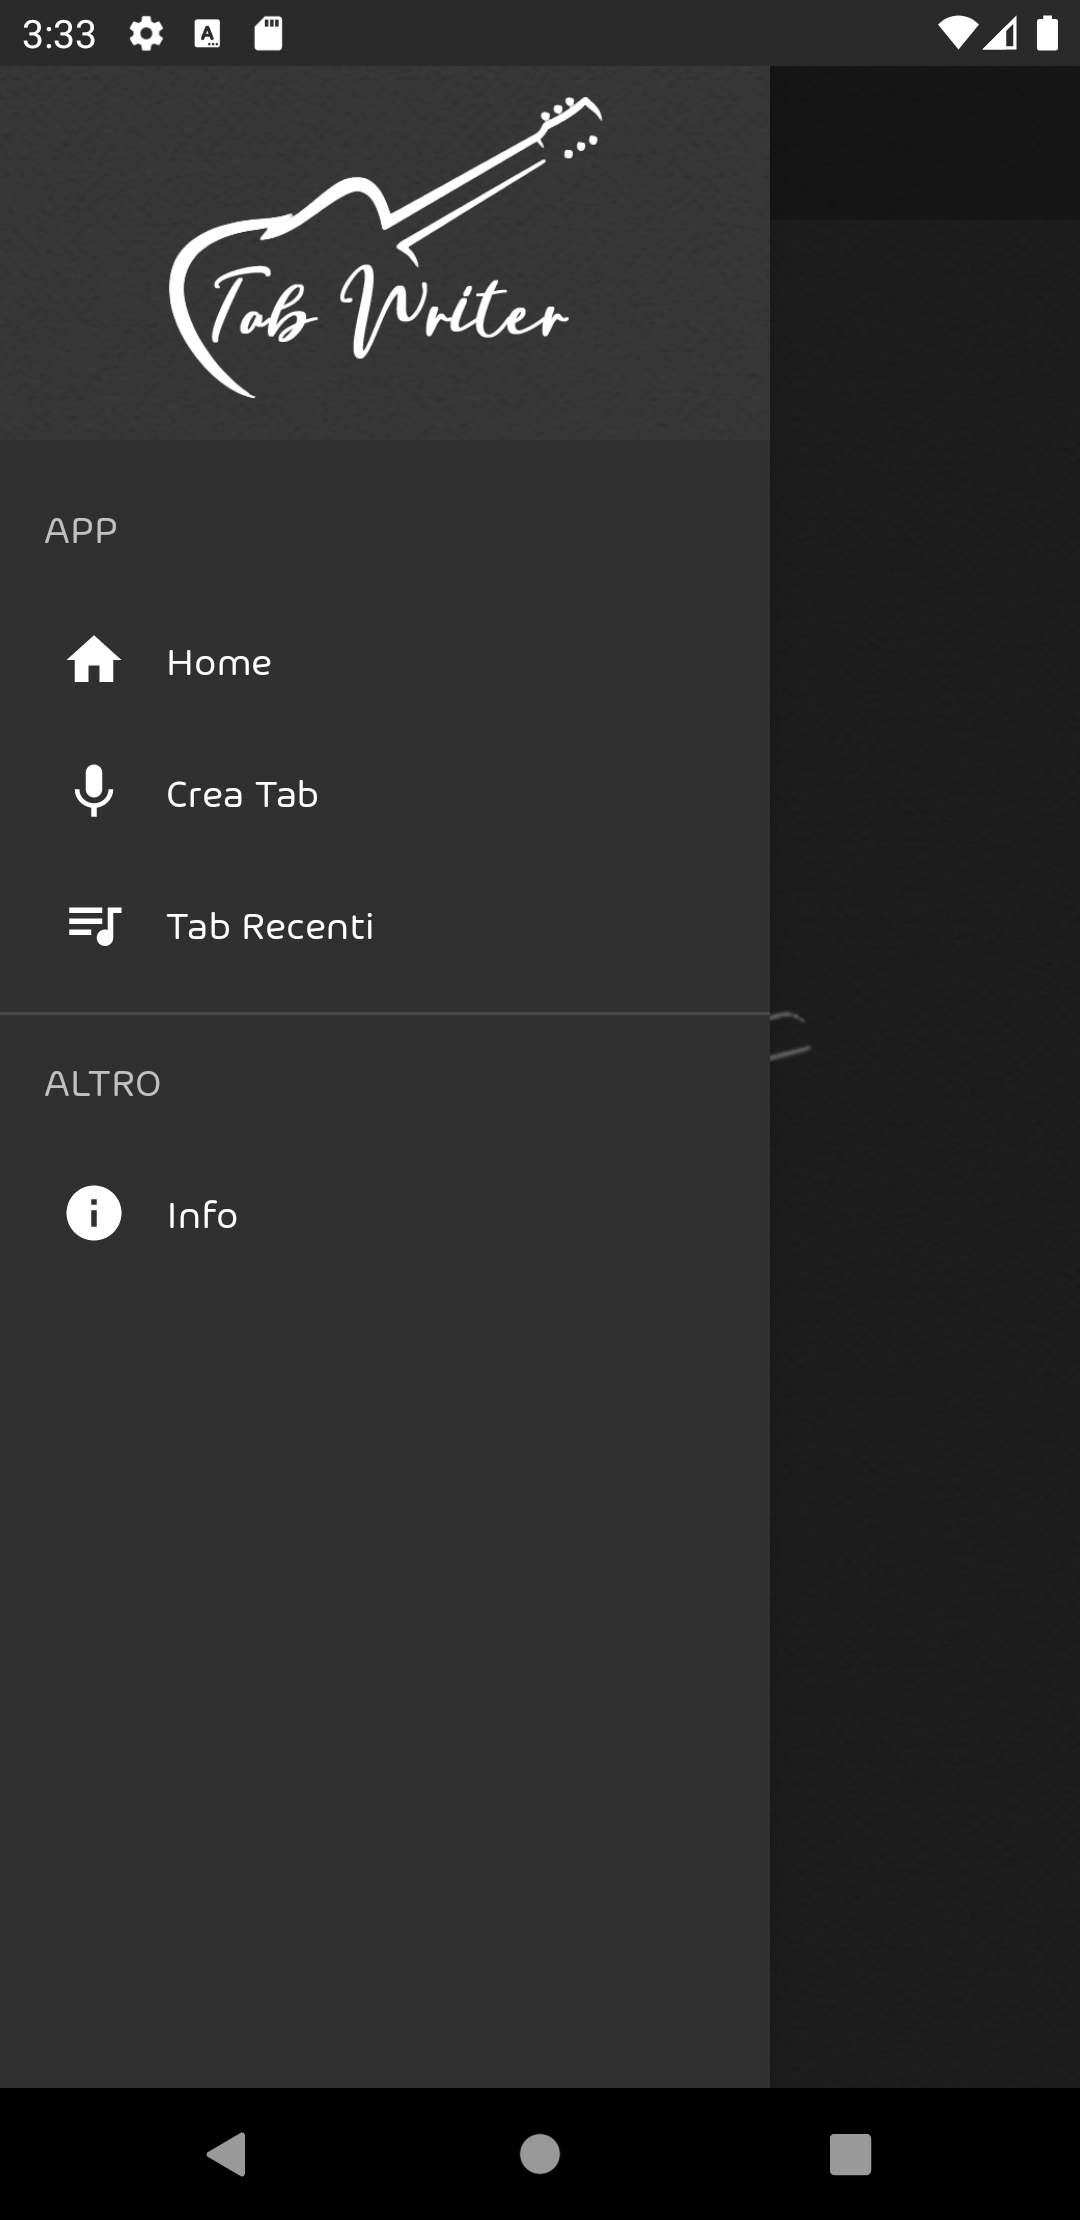
\includegraphics[scale=0.10]{./images/img17.png}
	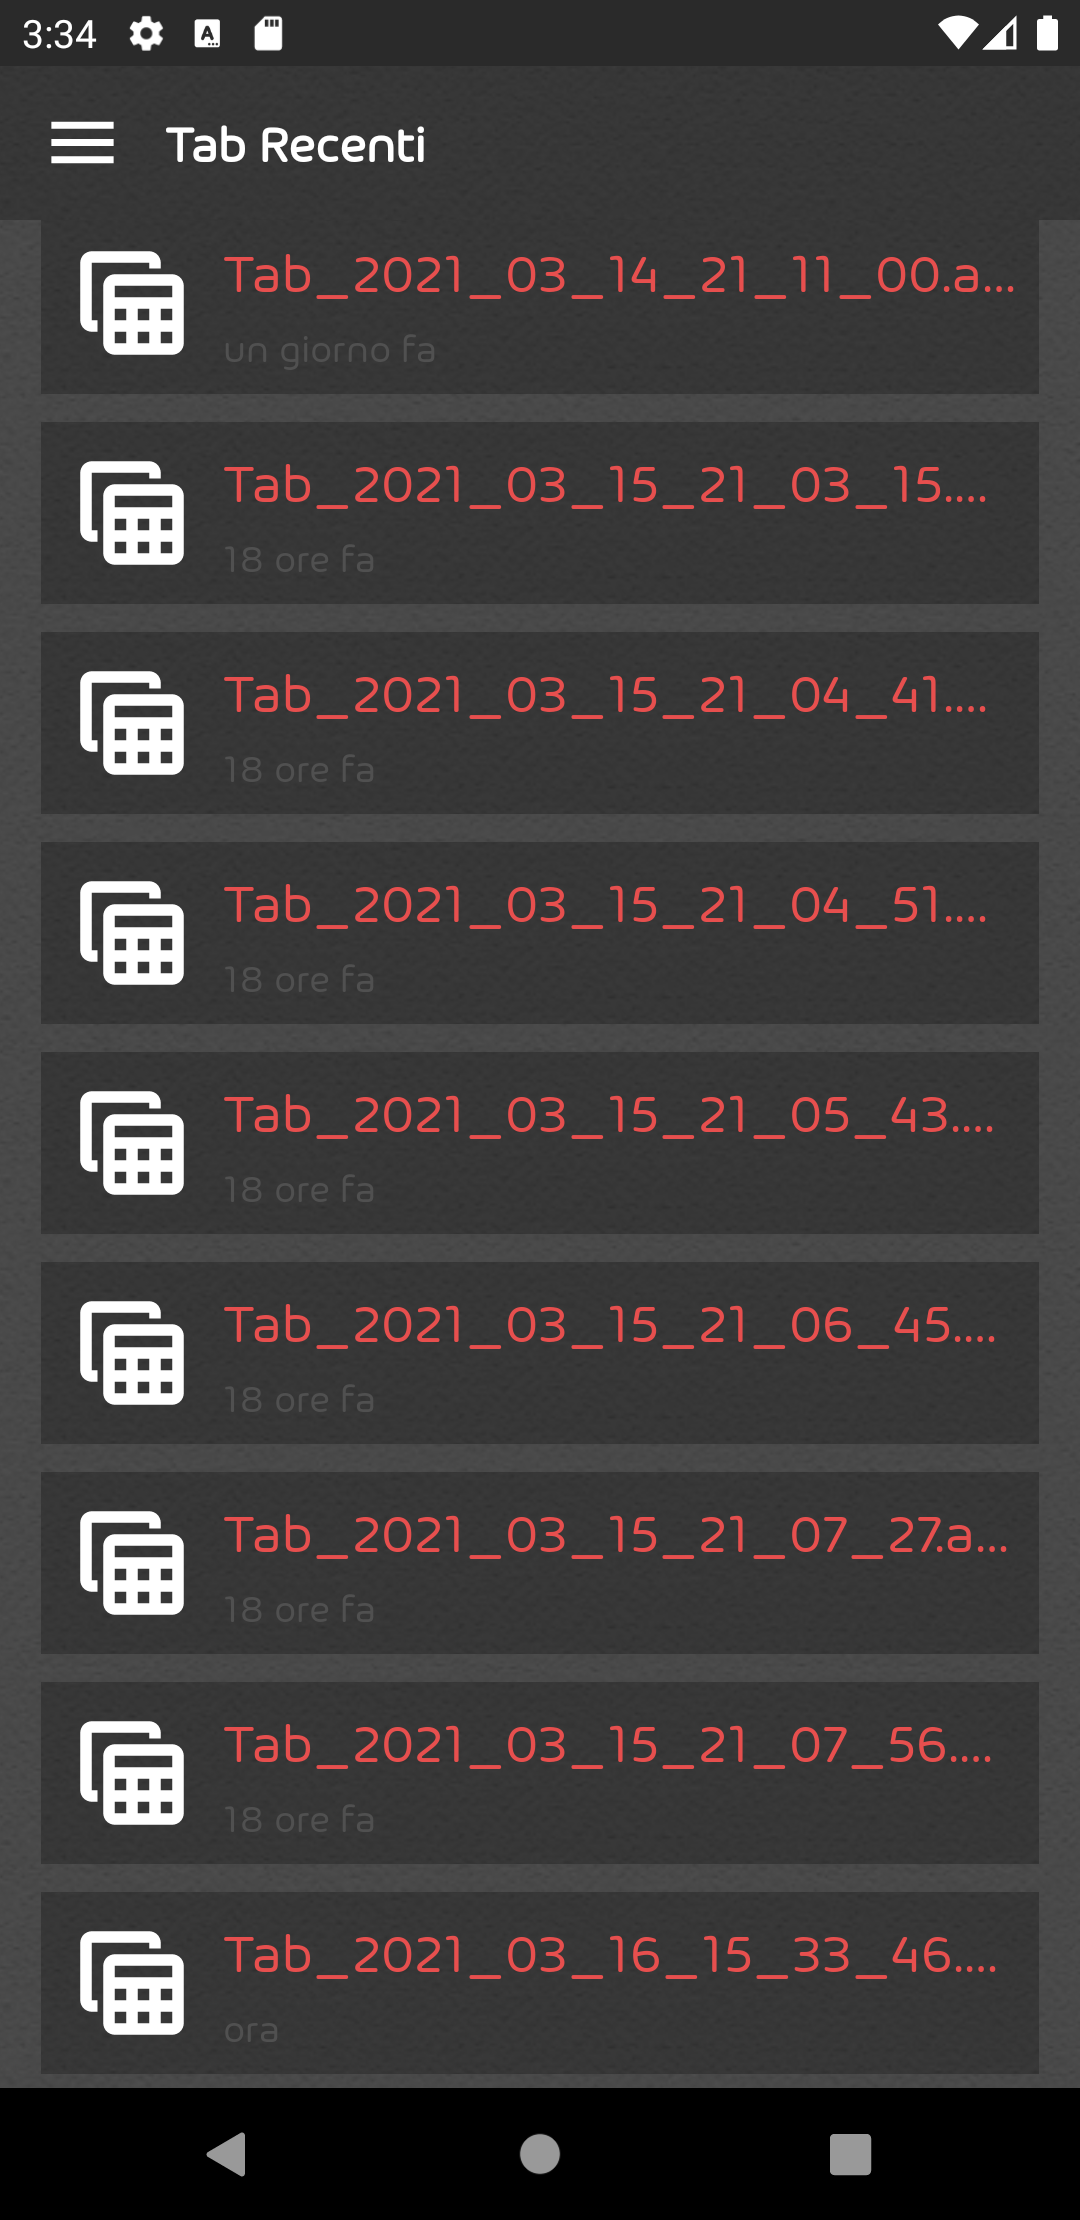
\includegraphics[scale=0.10]{./images/img20.png}
\end{figure}
\noindent Dopo aver creato le interfacce con gli elementi grafici, sia in \textit{light mode} che in \textit{dark mode}, è stato implementato un \textit{database} che tiene traccia delle \textit{tab} registrate e predette, in modo da poterle consultare anche in un secondo momento senza dover richiamare l'interprete di \textit{Tensorflow Lite}.\\
\newline
Per avviare la registrazione, basta cliccare sull'immagine centrale su cui c'è un microfono. A questo punto il cellulare registra il \textit{file} audio e per terminarla bisogna ricliccare sull'immagine.
\begin{figure}[H]
	\centering
	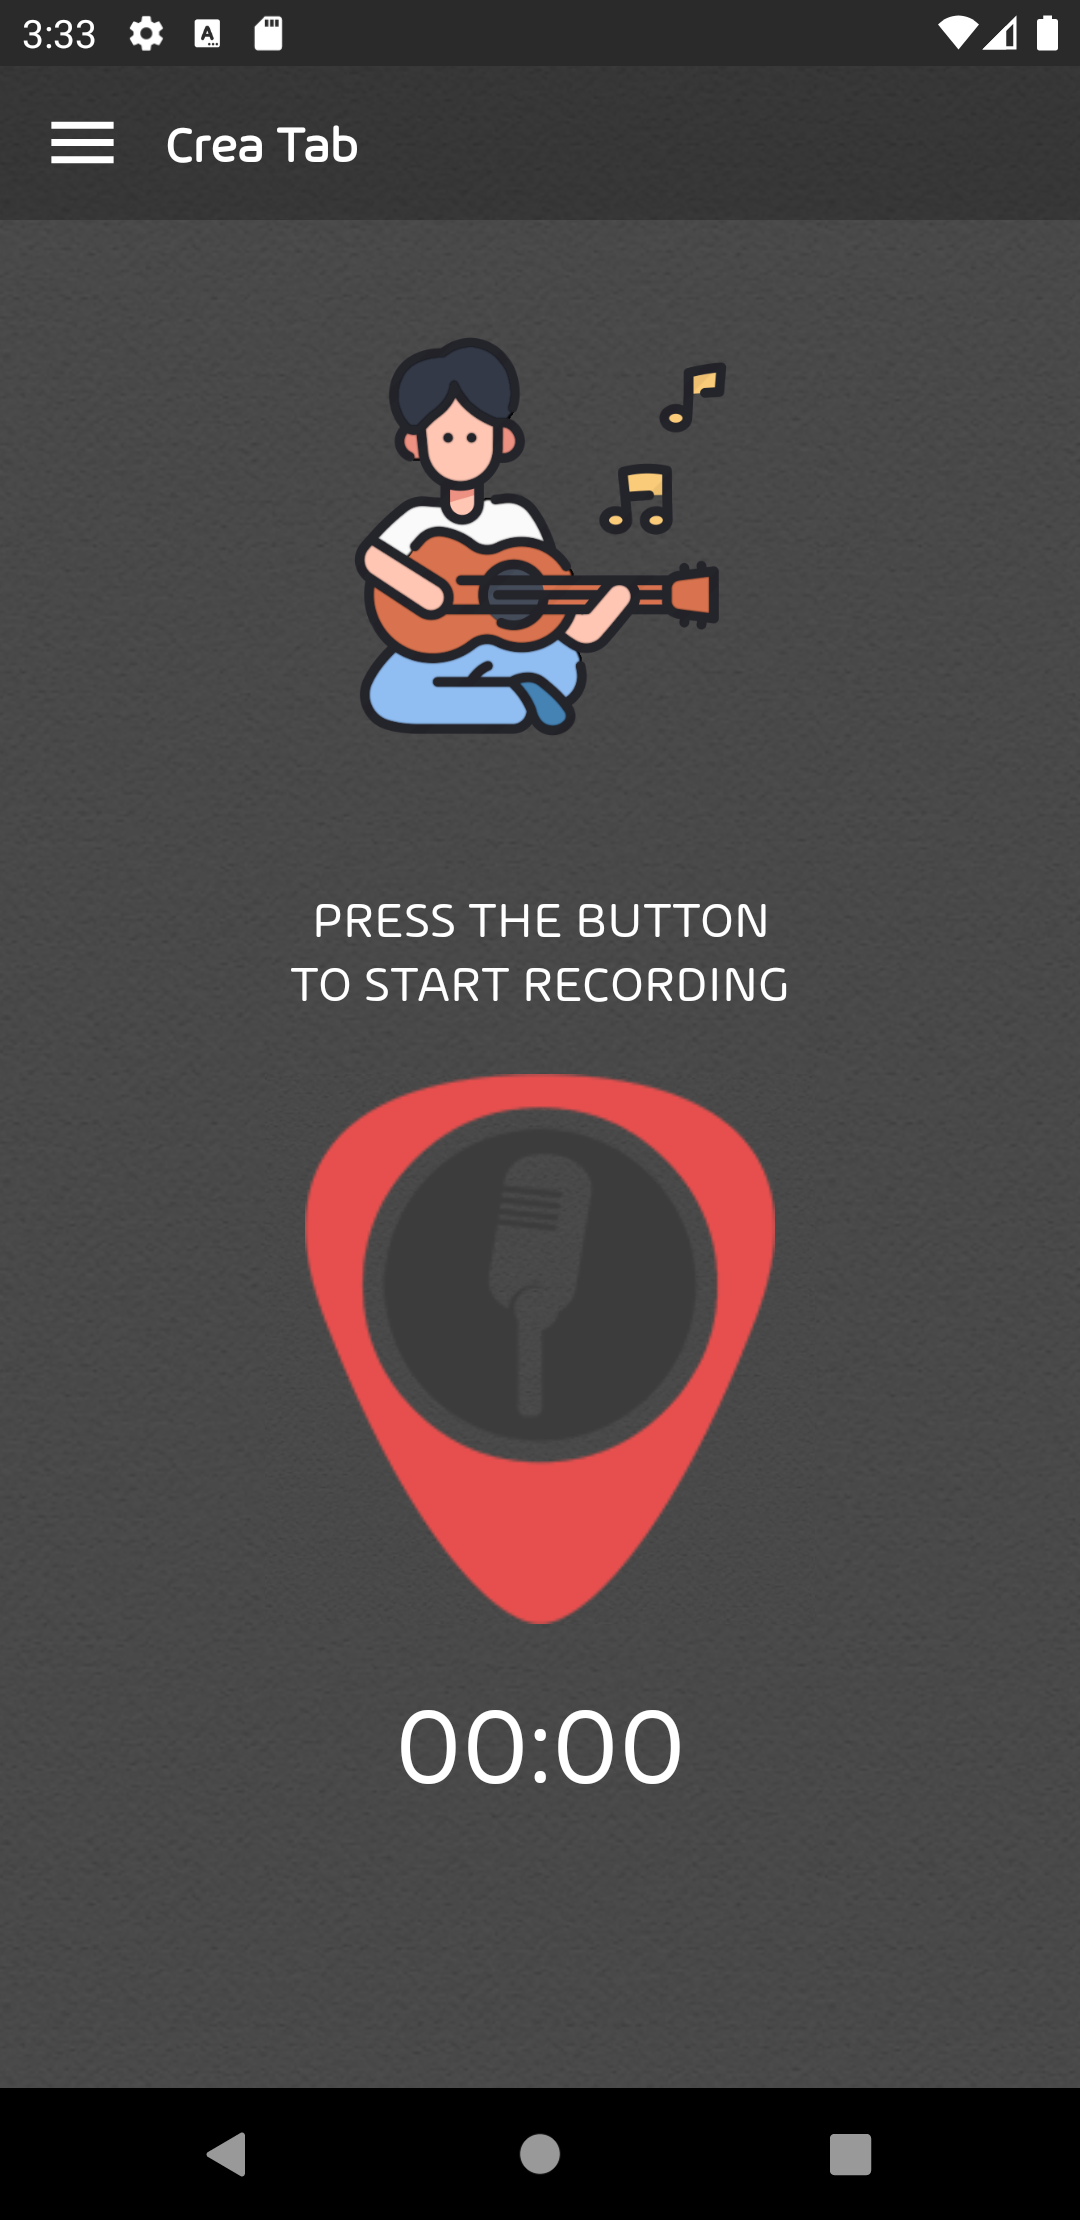
\includegraphics[scale=0.10]{./images/img18.png}
	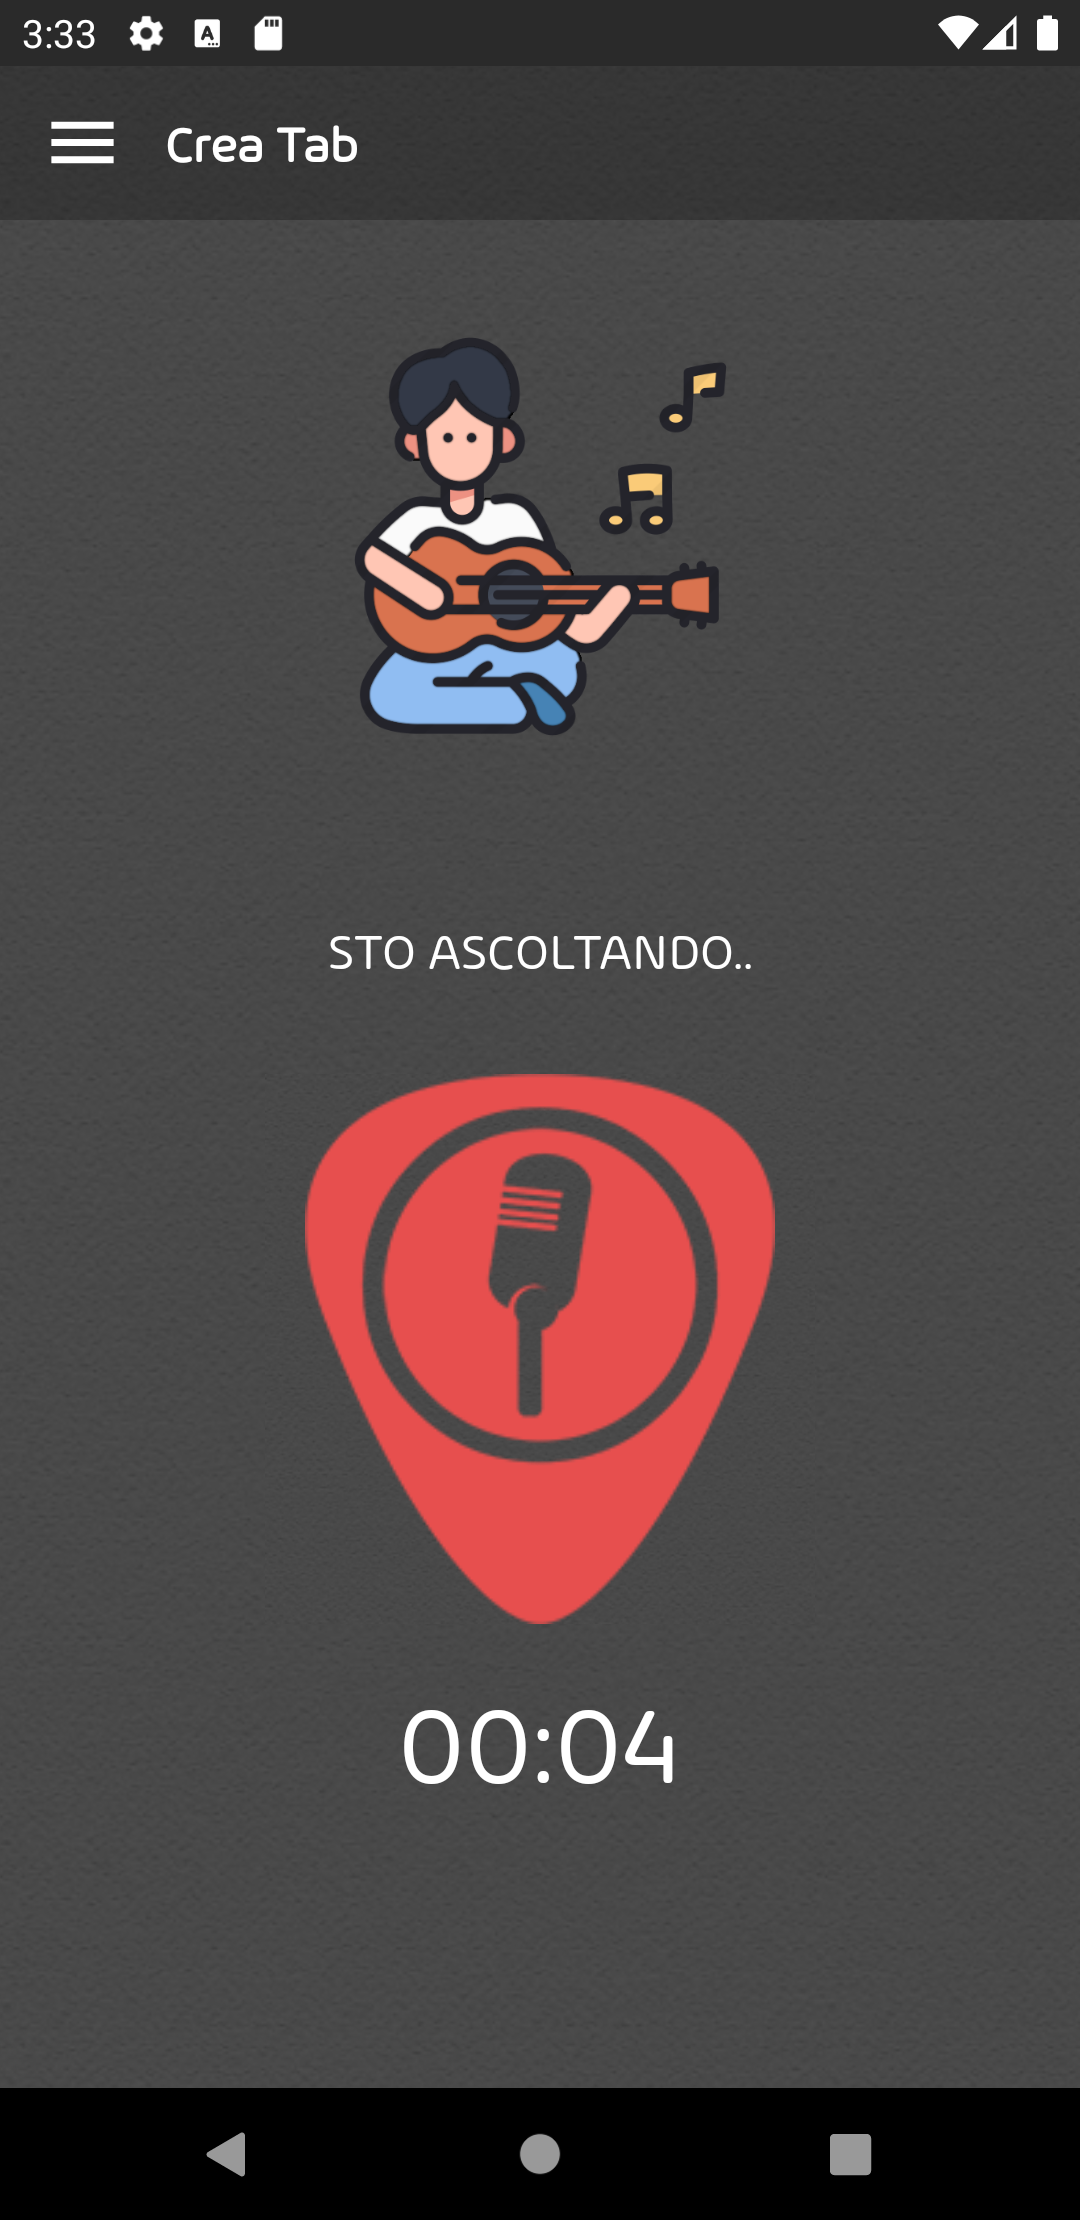
\includegraphics[scale=0.10]{./images/img22.png}
\end{figure}
\noindent A questo punto il file verrà salvato sul cellulare e convertito nel formato .\textit{wav} e grazie al modello della rete è possibile avviare la predizione. Il risultato apparirà in una nuova interfaccia:
\begin{figure}[H]
	\centering
	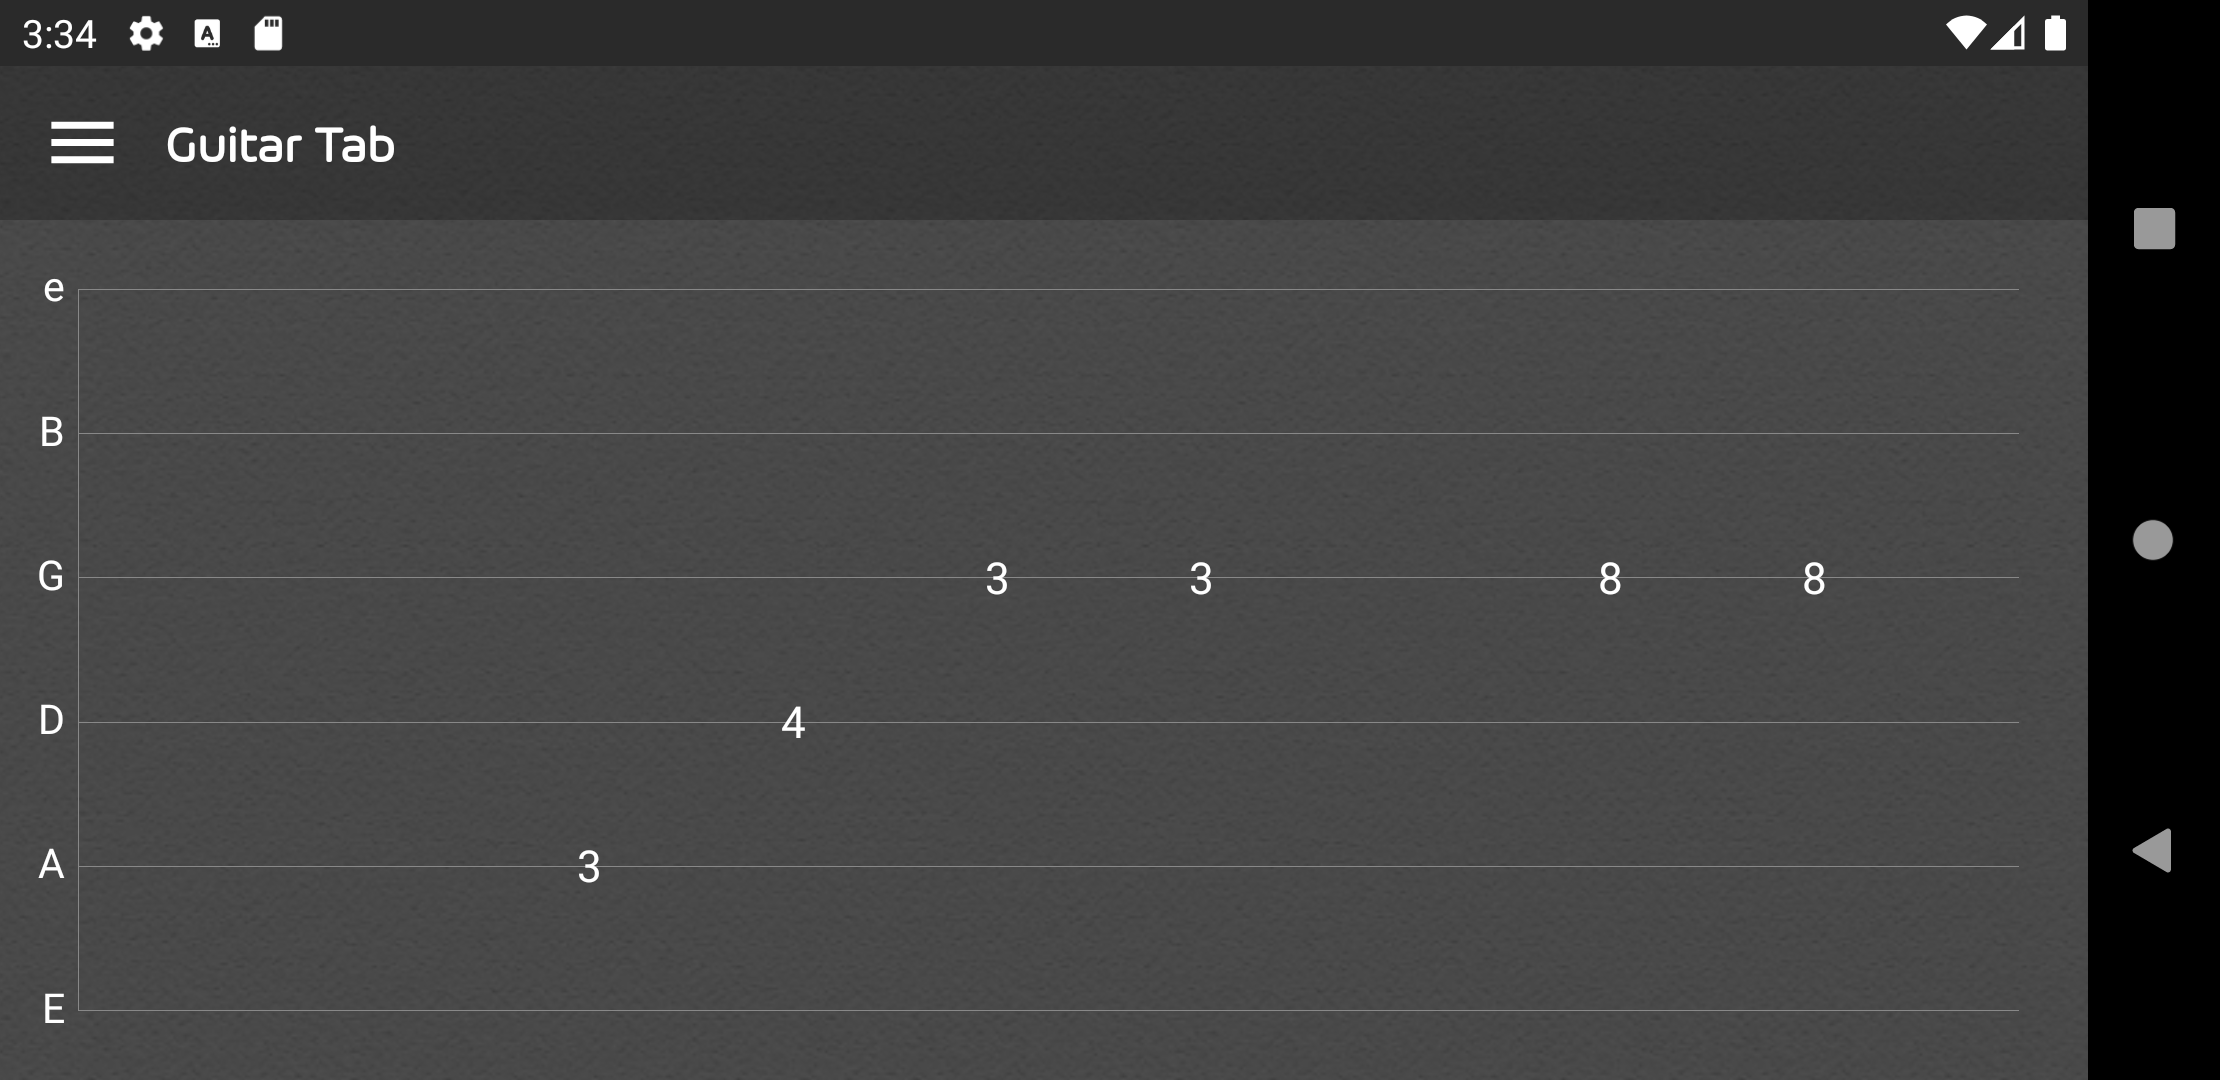
\includegraphics[scale=0.15]{./images/img19.png}
\end{figure}
\noindent \textbf{Problemi riscontrati:} putroppo non sono state trovate librerie in grado di ricavare, dal \textit{file} audio, la trasformata a Q costante come avevamo fatto su \textit{Python}.\\
\newline
%
\textbf{Soluzioni provate:}
\begin{itemize}
	\item Abbiamo pensato di utilizzare un \textit{server} che ricavi l'immagine della trasformata dall'audio registrato e la restituisca al dispositivo.\\
\end{itemize}
%
\textbf{Soluzione finale:} grazie ai ricevimenti fatti con il professore, ci è stato consigliato di usare \textit{chaquopy}, un \textit{plugin} che consente di implementare codice \textit{Python} all'interno delle applicazioni \textit{Android}.
\subsection{Pre-elaborazione dell'audio}
\textbf{Problemi riscontrati:} ricavando le immagini per ogni \textit{frame} di audio e successivamente facendo la \textit{predict} per ogni immagine, si ottenevano tante soluzioni quanti erano i \textit{frame}.\\ Per esempio, suonando il terzo tasto della quinta corda per due volte avremmo sull'interfaccia dell'applicazione una lunga serie di "3", perchè un \textit{frame} ha una durata di pochi millisecondi mentre la nota ha un \textit{range} di qualche secondo. La soluzione corretta sarebbe quella di avere solo due 3. \\
\newline
L'immagine sottostante fa vedere quanto è stato descritto:
\begin{figure}[H]
	\centering
	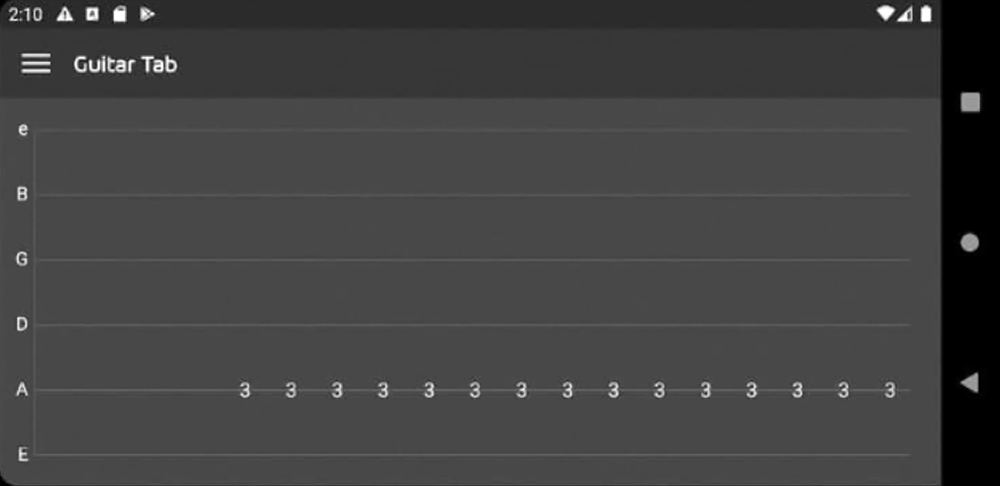
\includegraphics[scale=0.28]{./images/img25.png}
\end{figure}
\noindent \textbf{Soluzione finale:} visualizzando e analizzando lo spettrogramma, possiamo notare che quando una nota viene suonata ha un'ampiezza massima, come si può notare dal seguente grafico:
\begin{figure}[H]
	\centering
	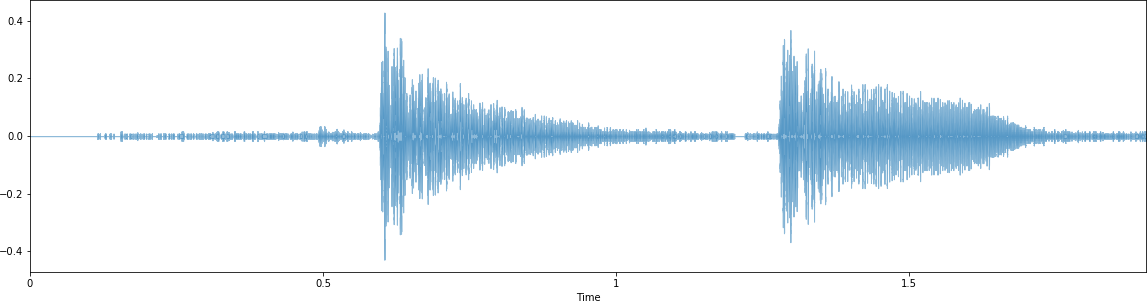
\includegraphics[scale=0.35]{./images/img26.png}
\end{figure}
\noindent Per trovare i punti, in questo caso due perchè è stata suonata due volte la stessa nota, ci viene in aiuto visualizzare l'\textit{RMS Energy} che è l'energia di un segnale. La funzione raggiunge il picco in due punti. In questo modo selezioniamo solo i \textit{frame} più significativi.
\begin{figure}[H]
	\centering
	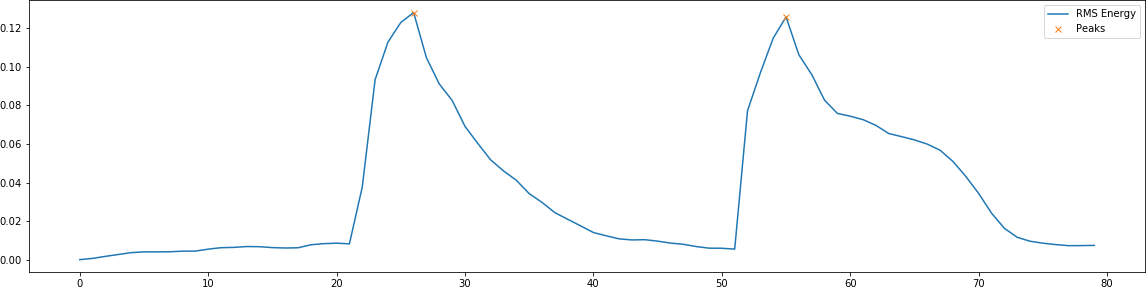
\includegraphics[scale=0.35]{./images/img27.png}
\end{figure}
\noindent Grazie alla funzione \textit{signal.find\_peaks()} della libreria \textit{scipy} troviamo tutti i massimi locali mediante un semplice confronto con i valori vicini in modo da ottenere solo i frame più significativi.
\vspace*{2ex}
\pythonexternal{./codes/preprocessing.py}
\vspace*{2ex}
Di conseguenza, vedremo solo due volte il tasto "3":
\begin{figure}[H]
	\centering
	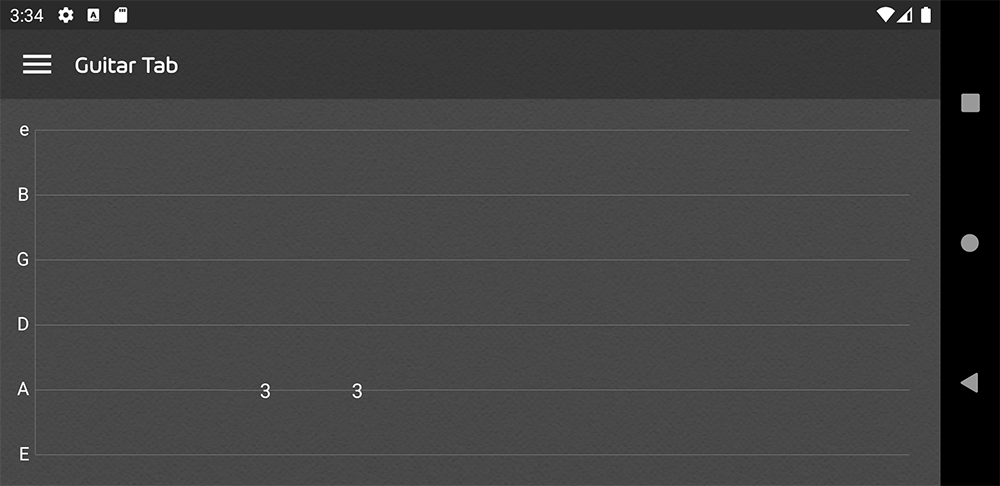
\includegraphics[scale=0.28]{./images/img24.png}
\end{figure}
\subsection{Implementazione di Tensorflow Lite}
Una volta ottenuti gli \textit{input} della rete possiamo eseguire l'inferenza con il modello. Inanzitutto rendiamo accessibile l'interprete di \textit{Tensorflow Lite}, allochiamo i tensori ed estrapoliamo dal modello rispettivamente il tipo e il formato dell'\textit{input} e dell'\textit{output}.\\ Solo i \textit{frame} più significativi verranno dati in \textit{input} all'interprete tramite la funzione \textit{interpreter.set\_tensor()}. Una volta che vengono definite le dimensione dell'\textit{input} e allocati i tensori, invochiamo l'interprete e tramite la funzione \textit{interpreter.get\_tensor()} otteniamo una copia dei valori provenienti dal tensore di \textit{output}. Infine, i risultati vengono salvati in un \textit{JSON} e conservati nel \textit{database} dell'applicazione.
\vspace*{2ex}
\pythonexternal{./codes/predict.py}
\section{Sviluppo applicazione iOS}
\subsection{Conversione del modello da Keras a CoreML}
Per poter usare il modello pre-addestrato sul cellulare abbiamo dovuto convertirlo nel formato \textit{.mlmodel} in modo da poter usare il \textit{framework Core ML}.\\
\newline
\textbf{Problemi riscontrati:} durante la conversione del modello sono apparsi diversi errori che impedivano la conversione. Gli errori sono simili a quello riportato di seguito:
\vspace*{2ex}
\textexternal{./codes/coreml.txt}
\vspace*{2ex}
\textbf{Soluzioni provate:}
\begin{itemize}
	\item Abbiamo preso spunto dal codice che si trova sul blocco di lucidi visti a lezione. Esso usa il \textit{package} \textit{tfcoreml}. Il focus dello \textit{script} è il seguente:
	\vspace*{2ex}
	\pythonexternal{./codes/coreml1.py}
	\vspace*{2ex}
	A questo punto serviva ottenere il file in formato \textit{.pb} da usare come \textit{input}. Questo file prende il nome di modello congelato. Prima di ottenerlo serve salvarci il modello che si ottiene con \textit{Tensorflow}. Esso è formato da quattro file:
	\begin{itemize}
		\item \textbf{model-ckpt.meta}: contiene il grafico completo (flusso di dati, le annotazioni per le variabili, le \textit{pipeline} di \textit{input} e altre informazioni);
     	\item \textbf{model-ckpt.data-0000-of-00001}: contiene tutti i valori delle variabili (pesi, segnaposto, gradienti, iperparametri, ecc.);
     	\item \textbf{model-ckpt.index}: ci sono tutti i metadati. È una tabella immutabile in cui ogni chiave è un nome di un tensore e il suo valore descrive i metadati di un tensore;
     	\item \textbf{checkpoint}: tutte le informazioni sul \textit{checkpoint}.
	\end{itemize}
	\vspace*{2ex}
	\pythonexternal{./codes/coreml2.py}
	\vspace*{2ex}
	\textit{estimator\_model.train()} serve a verificare che il modello esportato in precedenza sia effettivamente funzionante.\\
	\newline
	Il modello congelato ci consente di eliminare tutte le informazioni in più che vengono salvate perchè si potrebbe ricaricare quello appena salvato e l'addestramento continua da dove era stato interrotto.
	\vspace*{2ex}
	\pythonexternal{./codes/freezer.py}
	\vspace*{2ex}
	\item Uno dei nuovi tentativi si è basato sul cambio di codice per salvare il modello; abbiamo usato il seguente codice:
	\vspace*{2ex}
	\pythonexternal{./codes/coreml3.py}
	\vspace*{2ex}
	Tuttavia, i risultati non sono stati quelli sperati.
	
	\item Consultando la documentazione di \textit{coreml}, abbiamo scoperto che non sono previsti più aggiornamenti e consigliavano di usare un nuovo \textit{package}. Anche se fossimo stati in grado di convertirlo, non avremmo potuto utilizzare il modello su sistemi operativi \textit{iOS} maggiori di 12. La nuova libreria che abbiamo usato si chiama \textit{coremltools}.
	\vspace*{2ex}
	\pythonexternal{./codes/coremltools.py}
	\vspace*{2ex}
	\item Successivamente, per aumentare l'accuratezza, è stata inserita una funziona di attivazione personalizzata. Purtroppo, anche con \textit{coremltools} non siamo stati in grado di convertirlo perchè ci appariva un errore in corrispondenza del livello della nuova funzione:
	\vspace*{2ex}
	\textexternal{./codes/coremltools2.txt}
	\vspace*{2ex}
	
\end{itemize}
\textbf{Soluzione finale:} abbiamo deciso di usare \textit{Tensorflow Lite} perchè siamo riusciti a convertire il modello subito senza nessun problema.

\subsection{Sviluppo applicazione con Swift 5 e Xcode 12}
\textit{Swift} è un linguaggio di programmazione \textit{object-oriented} concepito per programmare sui sistemi operativi \textit{Apple}.\\
\newline
\textit{Xcode} è un ambiente di sviluppo integrato completamente sviluppato e mantenuto da \textit{Apple}, che consente di sviluppare \textit{software} per i sistemi \textit{macOS}, \textit{iOS}, \textit{watchOS} e \textit{tvOS}.\\
\newline
Abbiamo dovuto prendere un pò di familiarità con il nuovo linguaggio e il nuovo \textit{IDE} dato che non avevamo mai programmato nel mondo \textit{Apple}. La documentazione messa a disposizione agli sviluppatori è molto vasta e le solide basi apprese a ingegneria hanno fatto il resto.
La scelta è ricaduta direttamente sia all'ultima versione del linguaggio che dell'ambiente di sviluppo perché non avevamo vincoli sulla realizzazione dell'applicazione.\\
\newline
Le interfacce si realizzano in modo molto semplice perchè \textit{Xcode} consente di spostare gli elementi grafici con il \textit{mouse} e di posizionarli come si vuole. Tuttavia, è stata la parte che ha richiesto più tempo perchè li abbiamo dovuti configurare nel modo più adatto alle nostre esigenze.\\
\newline
E' stata prestata anche molta attenzione a rendere compatibile l'applicazione su modelli diversi. La dimensione dello schermo influisce molto sul \textit{layout} dell'applicazione. Senza le giuste modifiche è possibile che un elemento venga nascosto o spostato.
\begin{figure}[H]
	\centering
	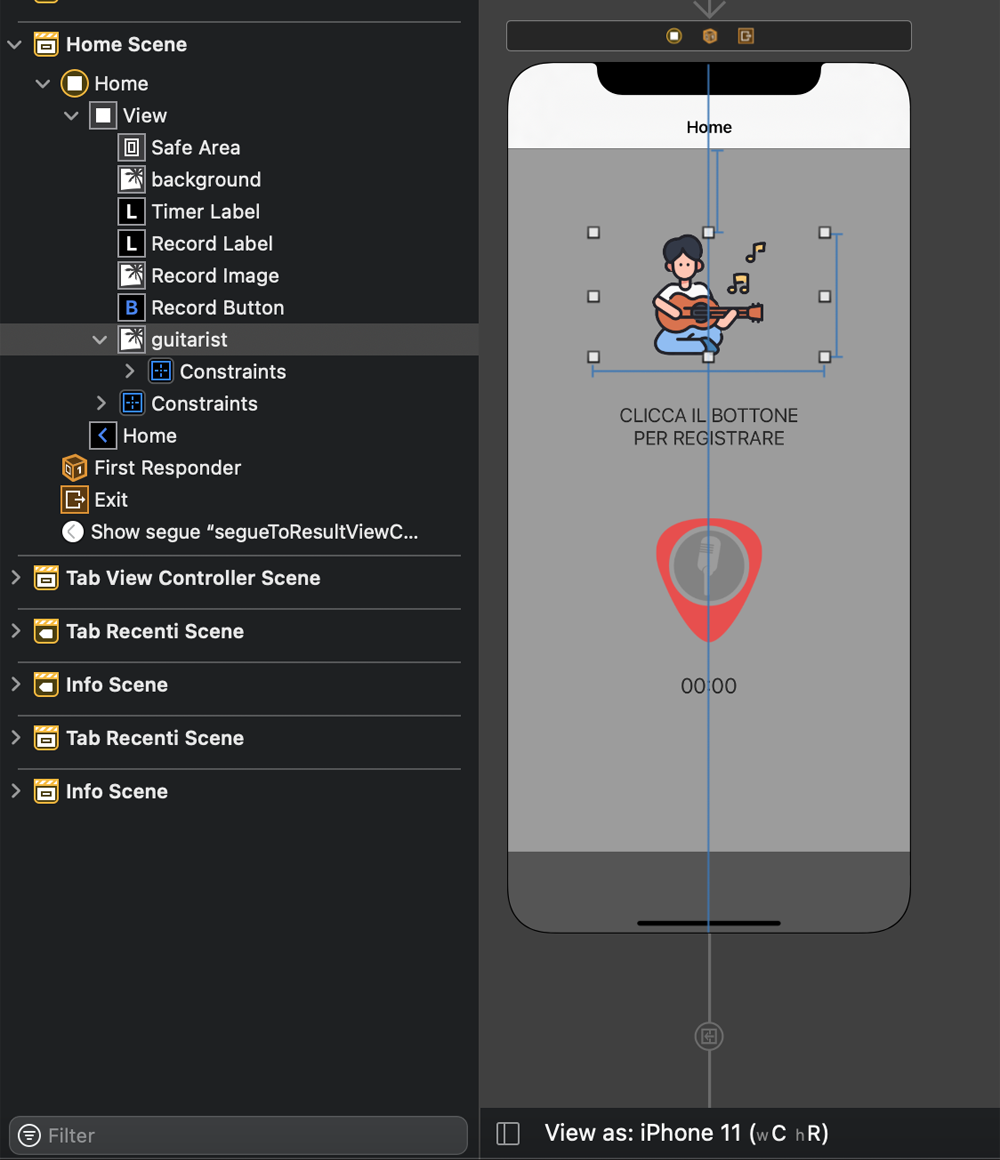
\includegraphics[scale=0.20]{./images/img2.png}
	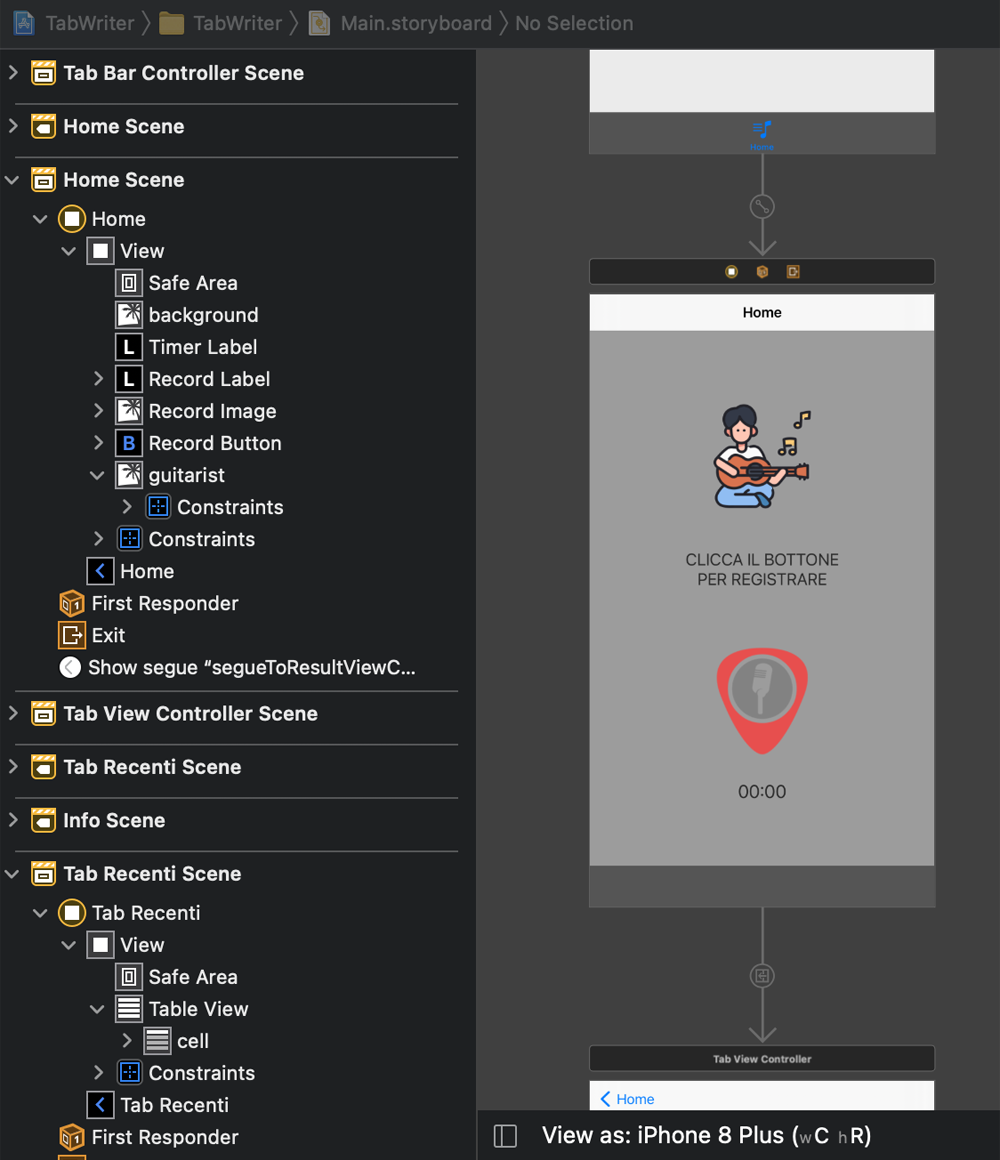
\includegraphics[scale=0.20]{./images/img3.png}
\end{figure}
\noindent Le due immagini precedenti mostrano chiaramente quello appena descritto: i due dispositivi sono diversi e le proporzioni vengono rispettate in entrambi.\\
\newline
L'applicazione che è stata realizzata da un punto di vista estetico è uguale a quella su \textit{iOS}. Cambiano solo leggeri particolari che differenziano i due mondi.\\
\newline
Inoltre, una particolare attenzione è stata dedicata anche sulla nuova modalità che sta riscontrando un grandissimo successo: la \textit{dark mode}. Dunque, sono stati presi tutti gli accorgimenti necessari per avere sia l'app compatibile con la versione chiara che con quella scura. L'immagine successiva mostra l'app in versione \textit{dark}:
\begin{figure}[H]
	\centering
	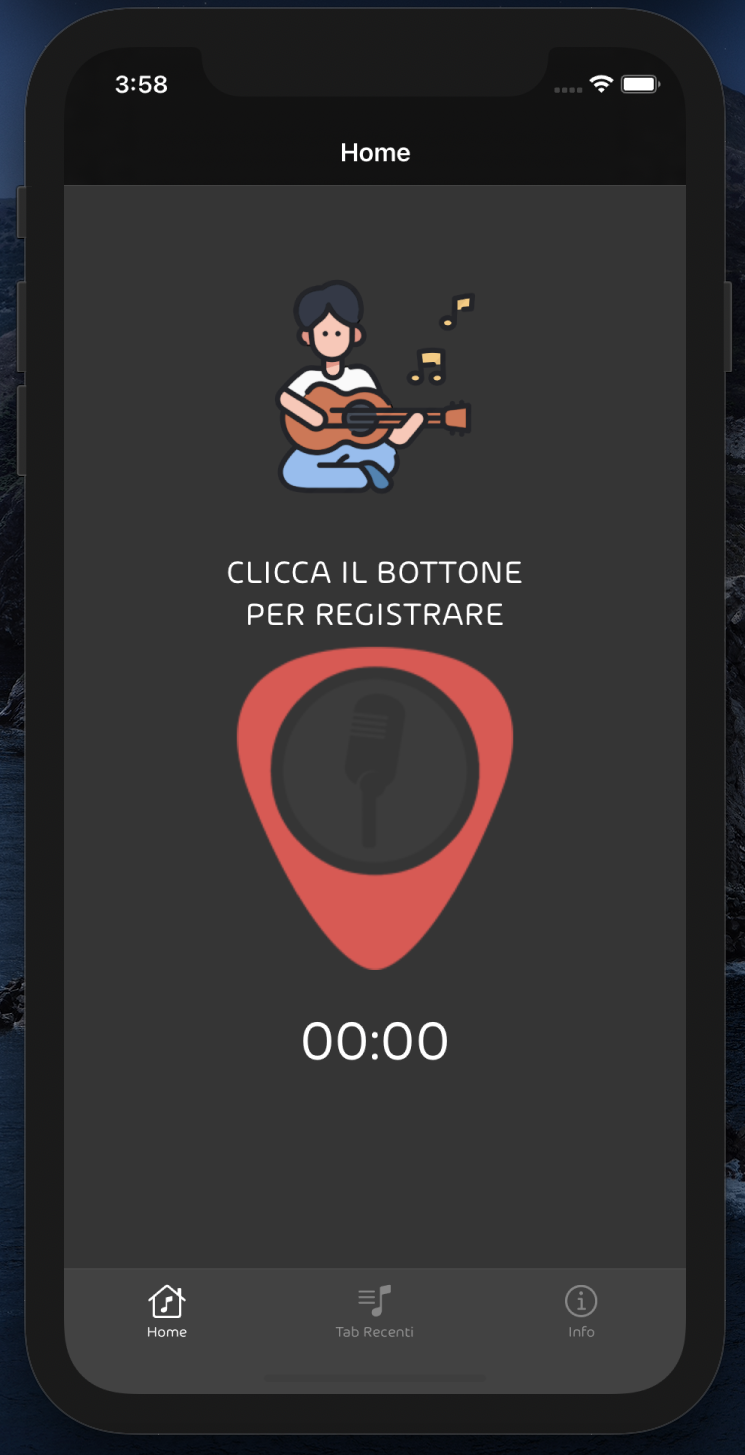
\includegraphics[scale=0.20]{./images/img10.png}
\end{figure}

\subsection{Uso di un server per l'uso della libreria librosa}
\textbf{Problemi riscontrati:} putroppo non sono state trovate librerie in grado di convertire il \textit{file} audio nella trasformata a Q costante.\\
\newline
%
\textbf{Soluzioni provate:}
\begin{itemize}
	\item Abbiamo provato ad usare la libreria \textit{PythonKit} senza successo perchè sui dispositivi \textit{iOS} manca l'interprete \textit{Python}.\\
\end{itemize}
%
\textbf{Soluzione finale:} per questo motivo ci siamo serviti di un \textit{server} che prende in ingresso la registrazione che è stata effettuata dallo \textit{smartphone} e restituisce in uscita le immagini del \textit{file} audio. Ovviamente la soluzione non è efficiente ma ai fini del progetto può andare più che bene. La predizione viene eseguita sul dispositivo e \textbf{non} sul \textit{server}.\\
\newline
Il \textit{server} è stato scritto grazie al \textit{micro-framework} \textit{Flask} scritto in \textit{Python}.
\vspace*{2ex}
\pythonexternal{./codes/flask.py}
\vspace*{2ex}
Le stesse operazioni descritte nel \textit{paragrafo 4.2.2} vengono eseguite dal \textit{server} che infatti ritorna solo i \textit{frame} più significativi.
\subsection{Implementazione di Tensorflow Lite}
Per utilizzare il nostro modello \textit{TensorFlow Lite} all'interno dell'applicazione, abbiamo dovuto prima configurare il progetto usando la libreria \textit{Firebase} e poi istanziato l'interprete per poterlo caricare. Nel seguente codice l'interprete viene istanziato grazie a \textit{Interpreter()}.
\vspace*{2ex}
\swiftexternal{./codes/tensorflowLiteIos1.swift}
\vspace*{2ex}
\noindent Per eseguire l'inferenza è necessario effettuare delle trasformazioni sui dati che sono obbligatorie per poterli dare in ingresso al modello. L'\textit{input} della rete deve essere un oggetto \textit{Data} al cui interno sono presenti i dati dell'\textit{array}contenente le immagini del \textit{file} audio (\textit{inputImages}).\\
A questo punto si allocano i tensori, si inserisce l'\textit{input} nella rete e si chiama il metodo \textit{invoke()}.
È possibile ottenere il tensore di \textit{output} chiamando il metodo \textit{output(at:)} e gli elementi ottenuti dalla predizione tramite \textit{output.data.copyBytes}. Inoltre, si può notare che ci sono due cicli: quello esterno serve per leggersi tutte le immagini della registrazione mentre il secondo funge da \textit{check} per verificare che l'immagine corrisponda a uno di quei picchi di cui abbiamo parlato in precedenza.
\vspace*{2ex}
\swiftexternal{./codes/tensorflowLiteIos2.swift}
\subsection{Installazione su dispositivo fisico}
L'applicazione è stata installata non solo sul simulatore ma anche sul dispositivo fisico. Lo \textit{smartphone} è un \textit{Iphone 11} con sistema operativo \textit{iOS} 14.1.
\begin{figure}[H]
	\centering
	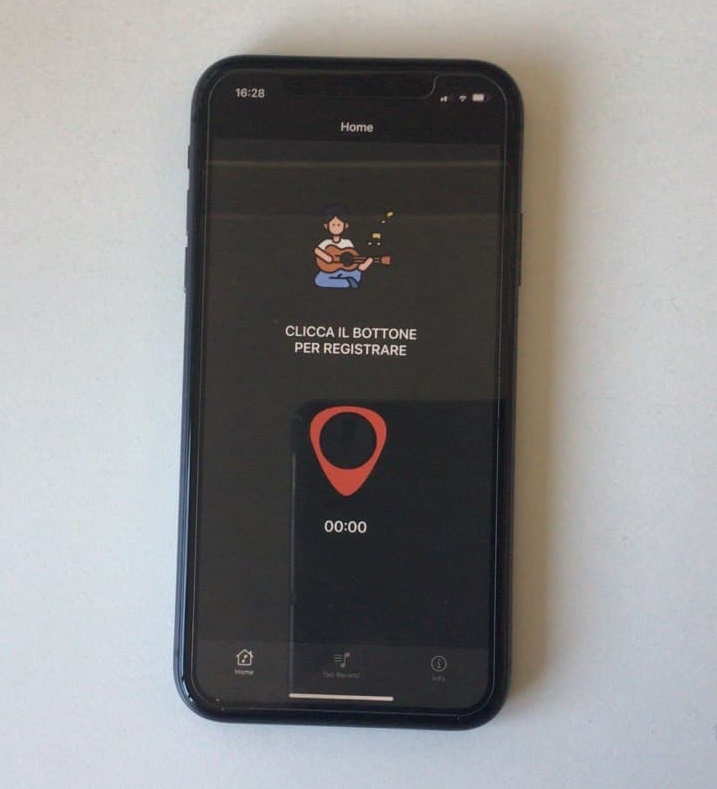
\includegraphics[scale=0.40]{./images/img21.jpg}
\end{figure}
    
    \chapter{Conclusioni}
    \label{CH:Concl}
    Sulle due applicazioni sono stati eseguiti diversi \textit{test} e possiamo affermare che si comportano entrambi abbastanza bene. Certamente, il progetto potrebbe essere migliorato perchè i limiti individuati sono i seguenti:
\begin{itemize}
		\item Se si suonassero ad esempio, le note 64 e 65 della prima corda in sequenza, la rete potrebbe predire una delle due note, o tutte e due, non sulla stessa corda ma in quella successiva. Questo non sarebbe un errore perchè il suono è lo stesso ma in certi casi sarebbe meglio suonare tasti vicini per una questione di manualità. Questo perchè il sistema determina la tablatura finestra per finestra e non tiene conto della sequenza della registrazione;
		\item Se la canzone è troppo veloce, cioè ha un tempo o BPM (battiti per minuto) alto, la predizione tende ad essere errata;
		\item Alcune note potrebbero non essere riconosciute perchè c'è ancora un margine di errore di quasi il 10\%.
	\end{itemize}
Nonostante ciò, siamo molto soddisfatti del progetto che è stato realizzato. Grazie a questa materia abbiamo esplorato due mondi che per noi erano sconosciuti come lo sviluppo di applicazioni \textit{mobile}. Siamo consapevoli che abbiamo perlustrato solo una piccola parte di questa vastissima materia ma quello che abbiamo appreso sarà sicuramente usato come base di partenza per progetti futuri.\\
\newline
A fini dimostrativi, forniamo insieme alla documentazione due brevi video delle applicazioni in funzione.
    
%     \nocite{*}
    \bibliographystyle{IEEEtran}
    %%%%%%%%%%% Example 1%%%%%%%%%%%%%%%%%%%%%%%%%%
    \begin{thebibliography}{100}  % 100 is a random guess of the total number of %references
    
    \bibitem{HK} \textit{Chitarra classica}. (s.d.). Wikipedia, l'enciclopedia libera. Ultimo accesso: 28 febbraio 2021, https://it.wikipedia.org/wiki/Chitarra
    
    \bibitem{HK} \textit{I tasti della chitarra}. (s.d.). TestoeAccordi. Ultimo accesso: 26 febbraio 2021, https://www.testoeaccordi.it/menu/tasti.htm
    
    \bibitem{HK} \textit{Note manico chitarra} [Image]. (s.d.). Videocorsochitarra. Ultimo accesso: 27 febbraio 2021, https://videocorsochitarra.it/note-manico-chitarra/
    
    \bibitem{HK} Savage. N. (s.d.). \textit{Come Leggere Tablature per Chitarra}. Wikihow. https://www.wikihow.it/Leggere-Tablature-per-Chitarra
    	
    \bibitem{Boney96} Q. Xi, R. Bittner, J. Pauwels, X. Ye, and J. P. Bello, "Guitarset: A Dataset for Guitar Transcription", \emph{in 19th International Society for Music Information Retrieval Conference}, Paris, France, Sept. 2018.
    
    \bibitem{MG} Note Frequency Chart (Download) [Image], Soundonsound.com, Dec 03, 2018 11:32 am.
    
     \bibitem{HK} \textit{Machine Learning e principio di funzionamento}. (s.d.). Lorenzo Govoni Business e Tecnologia Ultimo accesso: 24 marzo 2021, https://www.lorenzogovoni.com/machine-learning-e-funzionamento/
    
    \bibitem{HK} Drexel University, ExCITe Center, \emph{Expressive and Creative Interaction Technologies}, NEMISIG 2019
    
    \bibitem{HK} \textit{Utilizza un modello TensorFlow Lite per inferenza con ML Kit su iOS}. (s.d.). Firebase. Ultimo accesso: 03 marzo 2021, https://firebase.google.com/docs/ml-kit/ios/use-custom-models

	\end{thebibliography}
	%%%%%%%%%%%%% end %%%%%%%%%%%%%%%%%%%%%%%%%%%%%%%
\end{document}